\documentclass[10pt,paper=a4,headings=standardclasses
]{scrartcl}
\usepackage{mathpazo}
\usepackage{helvet}
\usepackage{amsmath}
\usepackage[total={6.75in, 9.5in}]{geometry}
\setlength{\parindent}{2em}
% use Unicode characters - try changing the option if you run into troubles with special characters (e.g. umlauts)
\usepackage[utf8]{inputenc}

% line numbers
\usepackage[right]{lineno}

% text layout - change as needed
% \raggedright

% Remove % for double line spacing
\usepackage{setspace} 
\doublespacing

% adjust caption style
\usepackage[aboveskip=1pt,labelfont=bf,labelsep=period,singlelinecheck=off]{caption}

% graphiccs and colours
\usepackage{graphicx,color}

% \RequirePackage{natbib}
\RequirePackage[authoryear,sort]{natbib}% uncomment this for author-year bibliography
% \RequirePackage{hyperref}
\usepackage[utf8]{inputenc} %unicode support
\usepackage{listings}
\definecolor{stringstyleCol}{rgb}{0.192,0.494,0.8}
\definecolor{NumCol}{rgb}{0.686,0.059,0.569}
\definecolor{basicstyleCol}{rgb}{0.345, 0.345, 0.345}
\lstdefinestyle{customR}{
  belowcaptionskip=1\baselineskip,
  captionpos=b,
  breaklines=true,
  numbers=left,
  frame=L,
  xleftmargin=\parindent,
  language=R,
  showstringspaces=false,
  basicstyle=\small\ttfamily\color{black},
%   keywordstyle=\bfseries\color{blue!40!black},
%   commentstyle=\itshape\color{purple!40!black},
%   identifierstyle=\color{green!40!black},
%   stringstyle=\color{red}
%   keywordstyle=\color{keywordstyleCol},      % keyword style
  commentstyle=\color{commentstyleCol},   % comment style
  stringstyle=\color{stringstyleCol},      % string literal style
  literate=%
   *{0}{{{\color{NumCol}0}}}1
    {1}{{{\color{NumCol}1}}}1
    {2}{{{\color{NumCol}2}}}1
    {3}{{{\color{NumCol}3}}}1
    {4}{{{\color{NumCol}4}}}1
    {5}{{{\color{NumCol}5}}}1
    {6}{{{\color{NumCol}6}}}1
    {7}{{{\color{NumCol}7}}}1
    {8}{{{\color{NumCol}8}}}1
    {9}{{{\color{NumCol}9}}}1
}
\usepackage{ulem}
\graphicspath{ {./figures/} }
\usepackage{wrapfig}
\setlength\linenumbersep{1cm}
\renewcommand\linenumberfont{\normalfont\footnotesize\sffamily}

% \usepackage{fancyhdr}
% \pagestyle{fancy}
% \fancyhf{}
% \fancyhead[RE,LO]{Pre-Processing ATLAS Data}

% %command for custom margin size
% \def\changemargin#1#2{\list{}{\rightmargin#2\leftmargin#1}\item[]}
% \let\endchangemargin=\endlist

\title{A Guide to Pre-Processing High-Throughput Animal Tracking Data}
\date{}
\author{Pratik Rajan Gupte\textsuperscript{1, 2} \and 
Christine E. Beardsworth\textsuperscript{2} \and
Orr Spiegel\textsuperscript{3} \and
Emmanuel Lourie\textsuperscript{4} \and
Sivan Toledo\textsuperscript{5} \and
Ran Nathan\textsuperscript{4} \and
Allert I. Bijleveld\textsuperscript{2}}

% document begins here
\begin{document}
% \vspace*{0.35in}

% title goes here:
% {\Large
% {\sffamily \textbf\newline{A Guide to Pre-Processing High-Throughput Animal Tracking Data}}
% }
\maketitle

% \newline
% authors go here:

\begin{flushleft}
% Author 4\textsuperscript{x},
% Author 5\textsuperscript{x},
% Author 6\textsuperscript{x},
% Author 7\textsuperscript{x}
\bigskip
\textbf{1} Groningen Institute for Evolutionary Life Sciences, University of Groningen, The Netherlands.
\\
\textbf{2} Deptartment of Coastal Systems, NIOZ Royal Netherlands Institute for Sea Research, The Netherlands.
\\
\textbf{3} School of Zoology, Faculty of Life Sciences, Tel Aviv University, Tel Aviv 69978, Israel.
\\
\textbf{4} Movement Ecology Lab, Department of Ecology, Evolution, and Behavior, Alexander Silberman Institute of Life Sciences, The Hebrew University of Jerusalem, 91904 Jerusalem, Israel.
\\
\textbf{5} Blavatnik School of Computer Science, Tel Aviv University, Israel.
\\
\bigskip

\textbf{Correspondence Author}
\\
Pratik R. Gupte
\\
\textbf{Address}
\\
Groningen Institute for Evolutionary Life Sciences, 
\\
Nijenborgh 7/5172.0581 9747 AG Groningen
\\
The Netherlands.
\\
\textbf{Email}
\\
pratikgupte16@gmail.com OR p.r.gupte@rug.nl
\\
\textbf{ORCID}
\\
https://orcid.org/0000-0001-5294-7819
\\
\textbf{Running Headline}
\\
Cleaning high-throughput animal tracking data

\end{flushleft}

\newpage

% now start line numbers
\linenumbers

\section*{Abstract} % abstract
\noindent
\begin{enumerate}
    \item Modern, high-throughput animal tracking studies collect increasingly large volumes of data at very fine temporal scales.
    At these scales, location error can exceed the animal's step size, confounding inferences from tracking data.
    `Cleaning' the data to exclude positions with large location errors prior to analyses is one of the main ways movement ecologists deal with location errors.
    Cleaning data to reduce location error before making biological inferences is widely recommended, and ecologists routinely consider cleaned data to be the ground-truth.
    Nonetheless, uniform guidance on this crucial step is scarce.
    
    \item Cleaning high-throughput data must strike a balance between rejecting location errors without discarding valid animal movements.
    Additionally, users of high-throughput systems face challenges resulting from the high volume of data itself, since processing large data volumes is computationally intensive and difficult without a common set of efficient tools.
    Furthermore, many methods that cluster movement tracks for ecological inference are based on statistical phenomena, and may not be intuitive to understand in terms of the tracked animal's biology.
    
    \item In this article we introduce a pipeline to pre-process high-throughput animal tracking data in order to prepare it for subsequent analysis. 
    We demonstrate this pipeline on simulated movement data to which we have randomly added location errors.
    We further suggest how large volumes of cleaned data may be synthesized into biologically meaningful ‘residence patches’.
    We then use calibration data to show how the pipeline improves its quality, and to verify that the residence patch synthesis accurately captures animal space-use.
    Finally, turning to real tracking data from Egyptian fruit bats (\textit{Rousettus aegyptiacus}), we demonstrate the pre-processing pipeline and residence patch method in a fully worked out example.
    
    \item To help with fast implementations of our pipeline, and to help standardise methods, we developed the \texttt{R} package \texttt{atlastools}, which we introduce here.
    Our pre-processing pipeline and \texttt{atlastools} can be used with any high-throughput animal movement data in which the high data volume combined with knowledge of the tracked individuals’ biology can be used to reduce location errors.
    The use of common pre-processing steps that are simple yet robust promotes standardised methods in the field of movement ecology and better inferences from data.
\end{enumerate}

\textbf{Keywords} ATLAS, data cleaning, movement ecology, high-throughput tracking, \textit{R} package \textit{atlastools}, residence patch

\linenumbers

\section{Introduction}

Tracking individual animals is the methodological mainstay of movement ecology, which seeks to link animal movement with internal causes, environmental factors, and resulting consequences \citep{nathan2008a, holyoak2008}. 
Investigating fine-scale environmental and social drivers and the consequences of movement requires position data from many individuals at high temporal and spatial resolution.
Such high-throughput tracking is possible using GPS tags \citep[see recent examples in][]{strandburg-peshkin2015, papageorgiou2019, harel2016}, yet ‘reverse-GPS’ systems developed to track animals over land \citep{toledo2014, weiser2016, toledo2016,toledo2020, maccurdy2009, maccurdy2019} and in aquatic systems \citep{hussey2015, baktoft2019, baktoft2017,jung2015} routinely produce high-throughput tracking data at much lower costs.
Although high-resolution tracking inherently provides more detailed information about the true path of the tracked animal, high-throughput data presents a two-fold challenge to ecologists.
First, the location error of each position may approach or exceed the true step size of the animal compared to low-resolution tracking with the same measurement error.
This biases derived metrics such as speed and tortuosity \citep[see][]{ranacher2016, noonan2019, hurford2009, calenge2009}.
Additionally, the absolute location errors around a position introduces uncertainty when studying the location of an animal relative to fixed landscape features (e.g. roads) or mobile elements (e.g. other tracked individuals).
Users have two main options to improve data quality: making inferences after modelling the system-specific location error \citep{fleming2014a, fleming2020, jonsen2003, jonsen2005, johnson2008, patterson2008}, or pre-processing data to clean it of positions with large location errors \citep{bjorneraas2010}.
The first approach may be limited by the animal movement models it can fit to the data \citep{fleming2014a, noonan2019, fleming2020}, and may be beyond the computational capacity of common hardware, leading users to prefer data cleaning instead.
When attempting data cleaning, the second challenge of high-throughput tracking reveals itself: the large number of observations themselves \citep{weiser2016, toledo2020}.
Having large volumes of data to clean makes manual identification and removal of errors from individual tracks prohibitively time consuming, incentivising automation based on a protocol.

Pre-processing steps must justifiably discard large location errors, also called outliers, from tracks (analogous to reducing false positives) while avoiding the overzealous rejection of valid animal movements (analogous to reducing false negatives).
How well researchers balance these imperatives has consequences for downstream analyses \citep{stine2001}.
For instance, small-scale resource selection functions can easily infer spurious preference and avoidance effects when there is uncertainty about an animal's true position and movement \citep{visscher2006}.
Ecologists recognise that tracking data are imperfect observations of the underlying process of animal movement, yet they implicitly consider cleaned data equivalent to be the ground-truth.
This assumption is reflected by popular statistical methods in movement ecology such as Hidden Markov Models (HMMs) \citep{langrock2012}, stationary-phase identification methods \citep{patin2020a}, or step-selection functions (SSFs) \citep{barnett2008, signer2017, avgar2016}, which expect low location errors relative to real animal movement (i.e., a high signal-to-noise ratio).
This makes the reproducible, standardised removal of location errors crucial to any animal tracking study.
While gross errors are often removed by positioning-system algorithms, ‘reasonable’ errors often remain to confront end users \citep{fischler1981, weiser2016, ranacher2016}.
Location errors may be exacerbated by the conditions of deployment, with systematic differences in location error among different landscape types  \citep[see][]{lewis2007, deon2002, frair2004}. 
% For instance, the physical features of an animal’s habitat such as hills or woodland may impede the transmissions of radio-telemetry tags (Beardsworth et al. \textit{in prep.}), while canopy cover can lead to location errors in GPS tracking \citep{lewis2007}.
Standardised pre-processing steps should thus be general enough to tackle animal movement data recovered from a range of environments.

Despite the importance and ubiquity of reducing location errors in tracking data, movement ecologists lack formal guidance on this crucial step.
Pre-processing protocols are often system-specific, or have limited availability, or may not be easily tractable for mainstream computing hardware and software.
Furthermore, filtering out positions on their location error estimates may not be sufficient to recover a good track estimate when location error does not correspond to biological realism in movement \citep{weiser2016, ranacher2016}.
This makes identifying and removing implausible movements from a track an important component of recovering true animal movement \citep{bjorneraas2010}.
Even after removing large location errors and evidently unrealistic movement, a track may comprise of positions that are distributed around the true animal location.
Discarding these positions as `untrue' would lead to excessive data loss, but treating them as `real' locations would lead to unrealistic estimates of metrics such as speed \citep{noonan2019}.
The large data-volumes of high-throughput tracking allow for a neat solution: tracks can be `smoothed' to reduce small location errors that have remained undetected.
This large data volume becomes a challenge when users seek to examine animal space-use in relation to relevant environmental covariates, such as the predictors of prolonged residence in an area \citep[see][]{bracis2018}.
First, statistical modelling using high-throughput data may suffer from pseudo-replication since both the response (e.g. step-length) and the predictors (e.g. resource landscape values) are spatio-temporally auto-correlated and hence non-independent \citep{aarts2008, fleming2014a,bijleveld2016, oudman2018, harel2016}.
Second, fitting statistical models to datasets with many millions of observations may require significant innovation in mainstream statistical software \citep[e.g. ][]{wood2015}, and users may instead want to reduce data volumes by thinning or clustering.

Here, we present a hands-on guide to pre-processing high-throughput tracking data, and demonstrate a relatively simple data cleaning pipeline to prepare these data for subsequent analyses (see Fig. 1). 
We take two important considerations into account, (1) that methods must be computationally efficient, and (2) that the pre-processing steps should be easily understood and reproduced.
With these in mind we have developed the \texttt{R} package \texttt{atlastools} \citep{gupte2020a, rcoreteam2020}, which implements important steps of the pre-processing pipeline.
\texttt{R} is the computational environment of choice in movement ecology \citep{joo2020} and formalising tools as an \texttt{R} package improves portability and reproducibility \citep{marwick2018}.
\texttt{atlastools} functions are easy to use and understand, and rely on the efficiency of the \texttt{R} package \texttt{data.table} \citep{dowle2020}.
We begin by showing how the pipeline can clean simulated tracks to which we have artificially introduced location error \citep{gurarie2017}.
Beginning with basic spatio-temporal filtering of positions, we cover filtering movement tracks, and reducing the effect of location error with a median smooth.
Then, we suggest one solution to issues of computational tractability, which is to synthesise residence patches \citep[\textit{sensu}][]{bijleveld2016, oudman2018, barraquand2008} from clusters of spatio-temporally proximate positions, and so reveal important aspects of animal space use.
Using calibration data from a manually transported ATLAS tag, we demonstrate how the residence patch method in \texttt{atlastools} accurately identifies areas of prolonged residence under real field conditions.
Finally, we turn to data from Egyptian fruit bats (\textit{Rousettus aegyptiacus}) tracked in the Hula Valley, Israel, to show a fully worked out example of the pre-processing pipeline and the residence patch method.

\begin{figure}
    \centering
    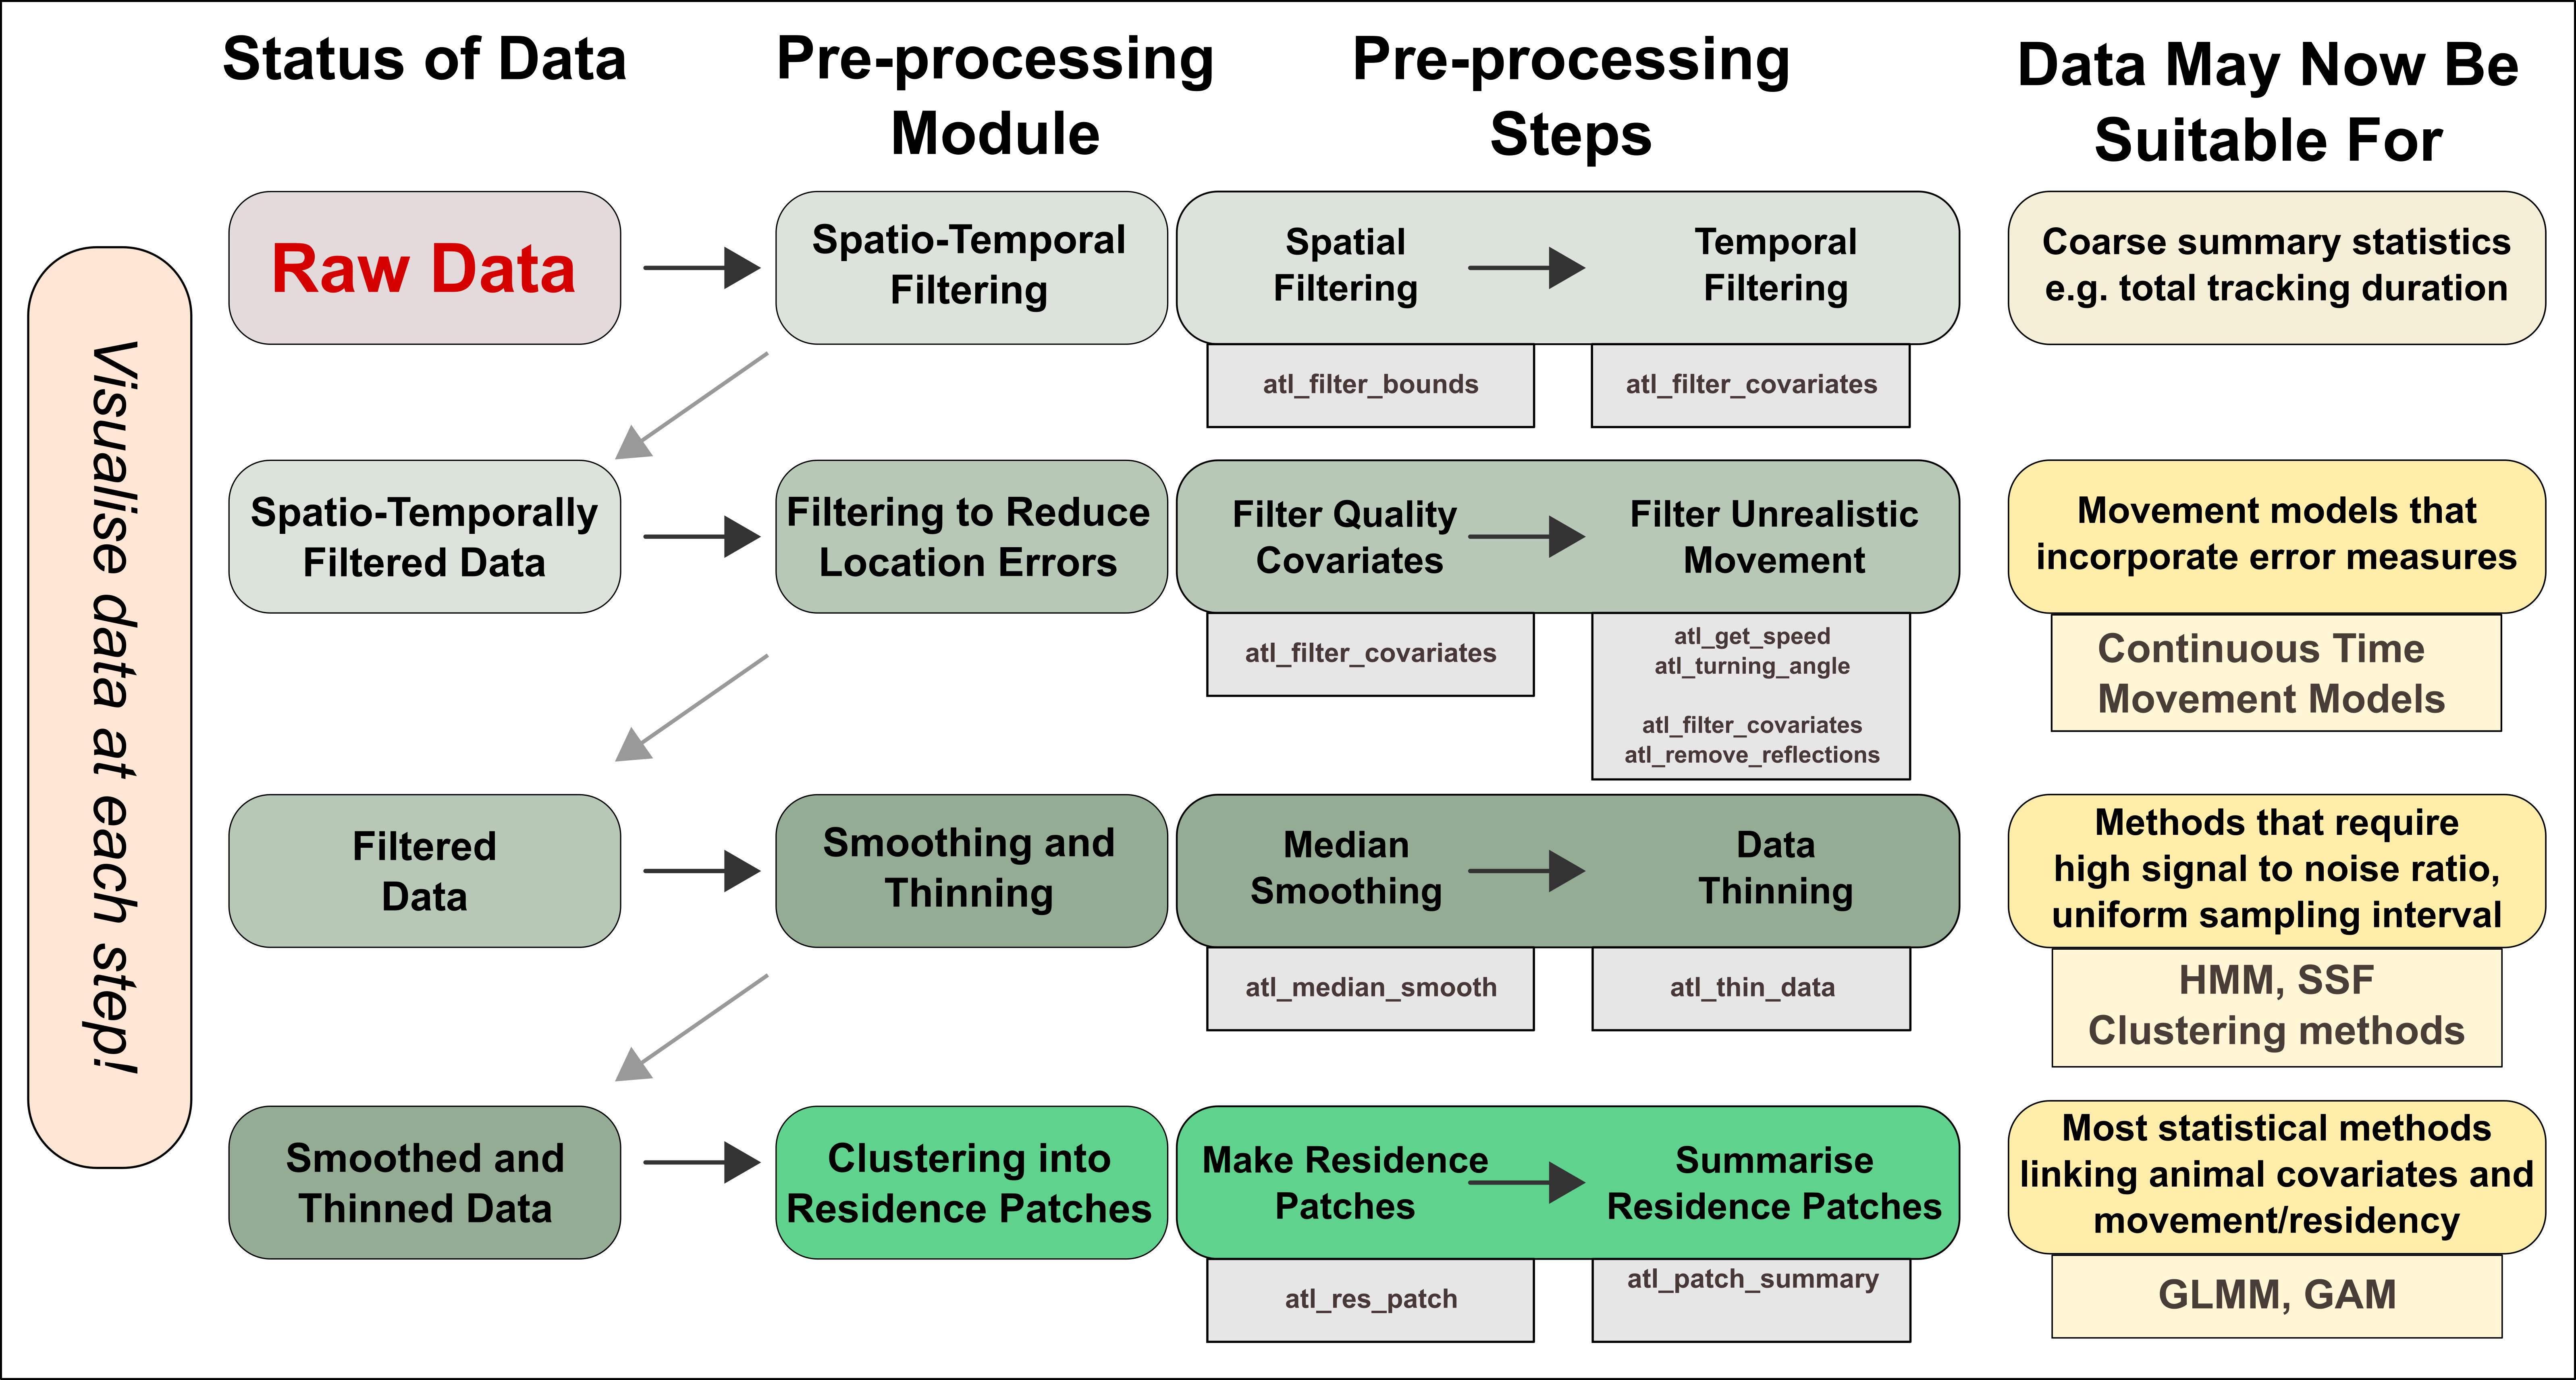
\includegraphics[width=0.99\textwidth]{figures/fig_01_recipe.png}
    \caption{A general, modular pipeline for pre-processing high-throughput tracking data from raw localisations to cleaned data, and optionally into residence patches. 
    Users should determine the appropriate pre-processing module, and work their way through the corresponding pre-processing steps, until the data are suitable for their intended purpose.
    The \texttt{atlastools} function that may be used to implement each pre-processing step is shown in the grey boxes underneath each step.
    Popular \texttt{R} packages in movement ecology, or statistical methods are shown underneath suggested analyses (yellow boxes).
    Users are strongly encouraged to visualise their data and scan it for location errors as a first step, and as they work through the pipeline.
    }
    \label{fig:figure_pipeline}
\end{figure}

\section{Pipeline Overview, Usage, and Simulating Data}

\subsection{The Pipeline and \texttt{atlastools}}

We lay out a modular pipeline for pre-processing raw high-throughput tracking data using the \texttt{R} package \texttt{atlastools} (Fig. 1).
While the pipeline and package were designed with ATLAS systems in mind, the principles and functions can be used with any high-throughput tracking data.
Users may follow the pipeline in full, or implement the module most suitable for their data.

\begin{enumerate}
    
    \item Users should visualise their data to check for evident location errors \citep{slingsby2016}.
    \item Users can install \texttt{atlastools} using the \texttt{install\_github} function from the \texttt{R} package \texttt{remotes}:
    
    \texttt{remotes::install\_github("pratikunterwegs/atlastools")}.
    
    Package functions are prefixed `\texttt{atl\_}', and are based on the \texttt{data.table} package (Dowle and Srinivasan 2020).
    Certain functions modify the input data "in place", and users must work on a copy of their data to preserve both the original and cleaned data (details in the Supplementary Material).
    Since high-throughput tracking systems typically cover an area of a few hundred square kilometres, \texttt{atlastools} users must convert their geographic coordinates to metres as this is assumed by all functions.
    \item Users can use simple spatio-temporal range filters to select positions within a certain time or area (see \textsc{Spatio-Temporal Filtering}).
    \item Next, users should reduce gross location errors by removing unreliable positions which may be identified by a system-specific error measure, or by the plausibility of associated movement metrics (see \textsc{Filtering to Reduce Location Errors}).
    \item Users should then reduce small-scale location errors by applying a median smooth (see \textsc{Smoothing and Thinning Data}).
    \item Users who need uniformly thinned data can either aggregate or resample it (see \textsc{Smoothing and Thinning Data}).
    At this stage, the data are ready for a number of popular statistical treatments such as Hidden Markov Model-based classification \citep{michelot2016,langrock2012}.
    \item Finally, users wishing to study prolonged animal residence in an area can classify their data into residence patches based on the movement ecology of their study system, after filtering out non-stationary positions (see \textsc{Synthesising Movement Tracks into Residence Patches}).
    
\end{enumerate}

\subsection{Simulating Movement Tracks}

To demonstrate the pipeline, we simulated a realistic movement track of 5,000 positions (unbiased correlated velocity model; UCVM) using the \texttt{R} package \texttt{smoove} \citep[][see Fig. 2.a]{gurarie2017}.
We added three kinds of error to the simulated track: (1) normally distributed small-scale offsets to the X and Y coordinates independently, (2) normally distributed large-scale offsets to a random subset (0.5 \%) of the positions, and (3) large-scale displacement of a continuous sequence of 300 of the 5,000 positions (indices 500 -- 800) (Fig. 2.a).
To demonstrate the residence patch method, we chose to simulate three independent rotational/advective correlated velocity movement (RACVM) tracks of 500 positions each ($\omega$ = 7, initial velocity = 0.1, $\mu$ = 0; see Gurarie et al. 2017), and connected them together with a roughly linear path (see Fig. 6.a).
RACVM models approximate the tracks of soaring birds which circle on thermals over a relatively small area, and move between thermals \citep[`thermalling'; ][]{gurarie2017, harel2016}.
This complex track structure provides a suitable challenge for the residence patch method and helps to demonstrate its generality.

\section{Spatio-Temporal Filtering}

\subsection{Spatial Filtering Using Bounding Boxes and Polygons}

First, data can be filtered to exclude positions outside the spatial bounds of a study area.
This simply involves comparing position coordinates with the range of acceptable coordinates (the bounding box), and removing those positions outside them (Fig. 2.b; Listing 1). 
A bounding box filter retains data from within a subset of the tracking range without the need for a geospatial representation such as a shapefile.
This can help remove unreliable data from a tracking system that is less accurate beyond a certain range (e.g. ATLAS; Beardsworth et al. \textit{in prep.}).
In some special cases, users may wish to \textit{remove} positions inside a bounding box, either because movement behaviour within an area is not the focus of a study, or because positions recorded within an area are known to be erroneous.
An example of the former is studies seeking to study transit behaviour between features which can be approximated by their bounding boxes. 
Instances of the latter are likely to be system specific, but are known from ATLAS systems (Bijleveld et al. \textit{in prep.}). 
One drawback to bounding box filters is that they are restricted to rectangular areas.
Users seeking to filter for areas with other geometries, such as a circular or irregular study area, need a geometric intersection between their data and a spatial representation of the area of interest (e.g. shapefile, geopackage, or \texttt{sf}-object in \texttt{R}).
The \texttt{atlastools} function \texttt{atl\_filter\_bounds} implements bounding box and explicit spatial filters and accepts X and Y coordinate ranges, an \texttt{sf}-polygon object \citep{pebesma2018}, or any combination of the three to filter the data (Listing 1).
Multipolygon objects are supported, allowing data from different areas to be selected.
When both coordinate ranges and a polygon are provided, the data is first filtered by the ranges and then the polygon.
The boolean function argument \texttt{remove\_inside} determines whether positions inside the bounds are retained (\texttt{FALSE}) or removed (\texttt{TRUE}).

\begin{lstlisting}[float,floatplacement=h!,language=R, style=customR, caption = {
    The \texttt{atl\_filter\_bounds} function removes positions outside an area defined by coordinate ranges, a polygon, or all three (\texttt{remove\_inside = FALSE}), or positions inside the area (\texttt{remove\_inside = TRUE}).
    The arguments \texttt{x} and \texttt{y} determine which columns are considered the X and Y coordinates, the arguments \texttt{x\_range} and \texttt{y\_range} determine the acceptable range of coordinates in a reference system based in metres, while the \texttt{sf\_polygon} argument allows the data to be filtered by the user specified \texttt{sf-(MULTI)POLYGON} object. 
    \texttt{atl\_filter\_bounds} returns a filtered \texttt{data.table}, which must be saved as an object (here, \texttt{filtered\_data}).}]
filtered_data <- atl_filter_bounds(data = data,
                    x = "X", y = "Y",
                    x_range = c(x_min, x_max),
                    y_range = c(y_min, y_max),
                    sf_polygon = your_polygon,
                    remove_inside = FALSE)
\end{lstlisting}

\begin{figure}[h!]
    \centering
    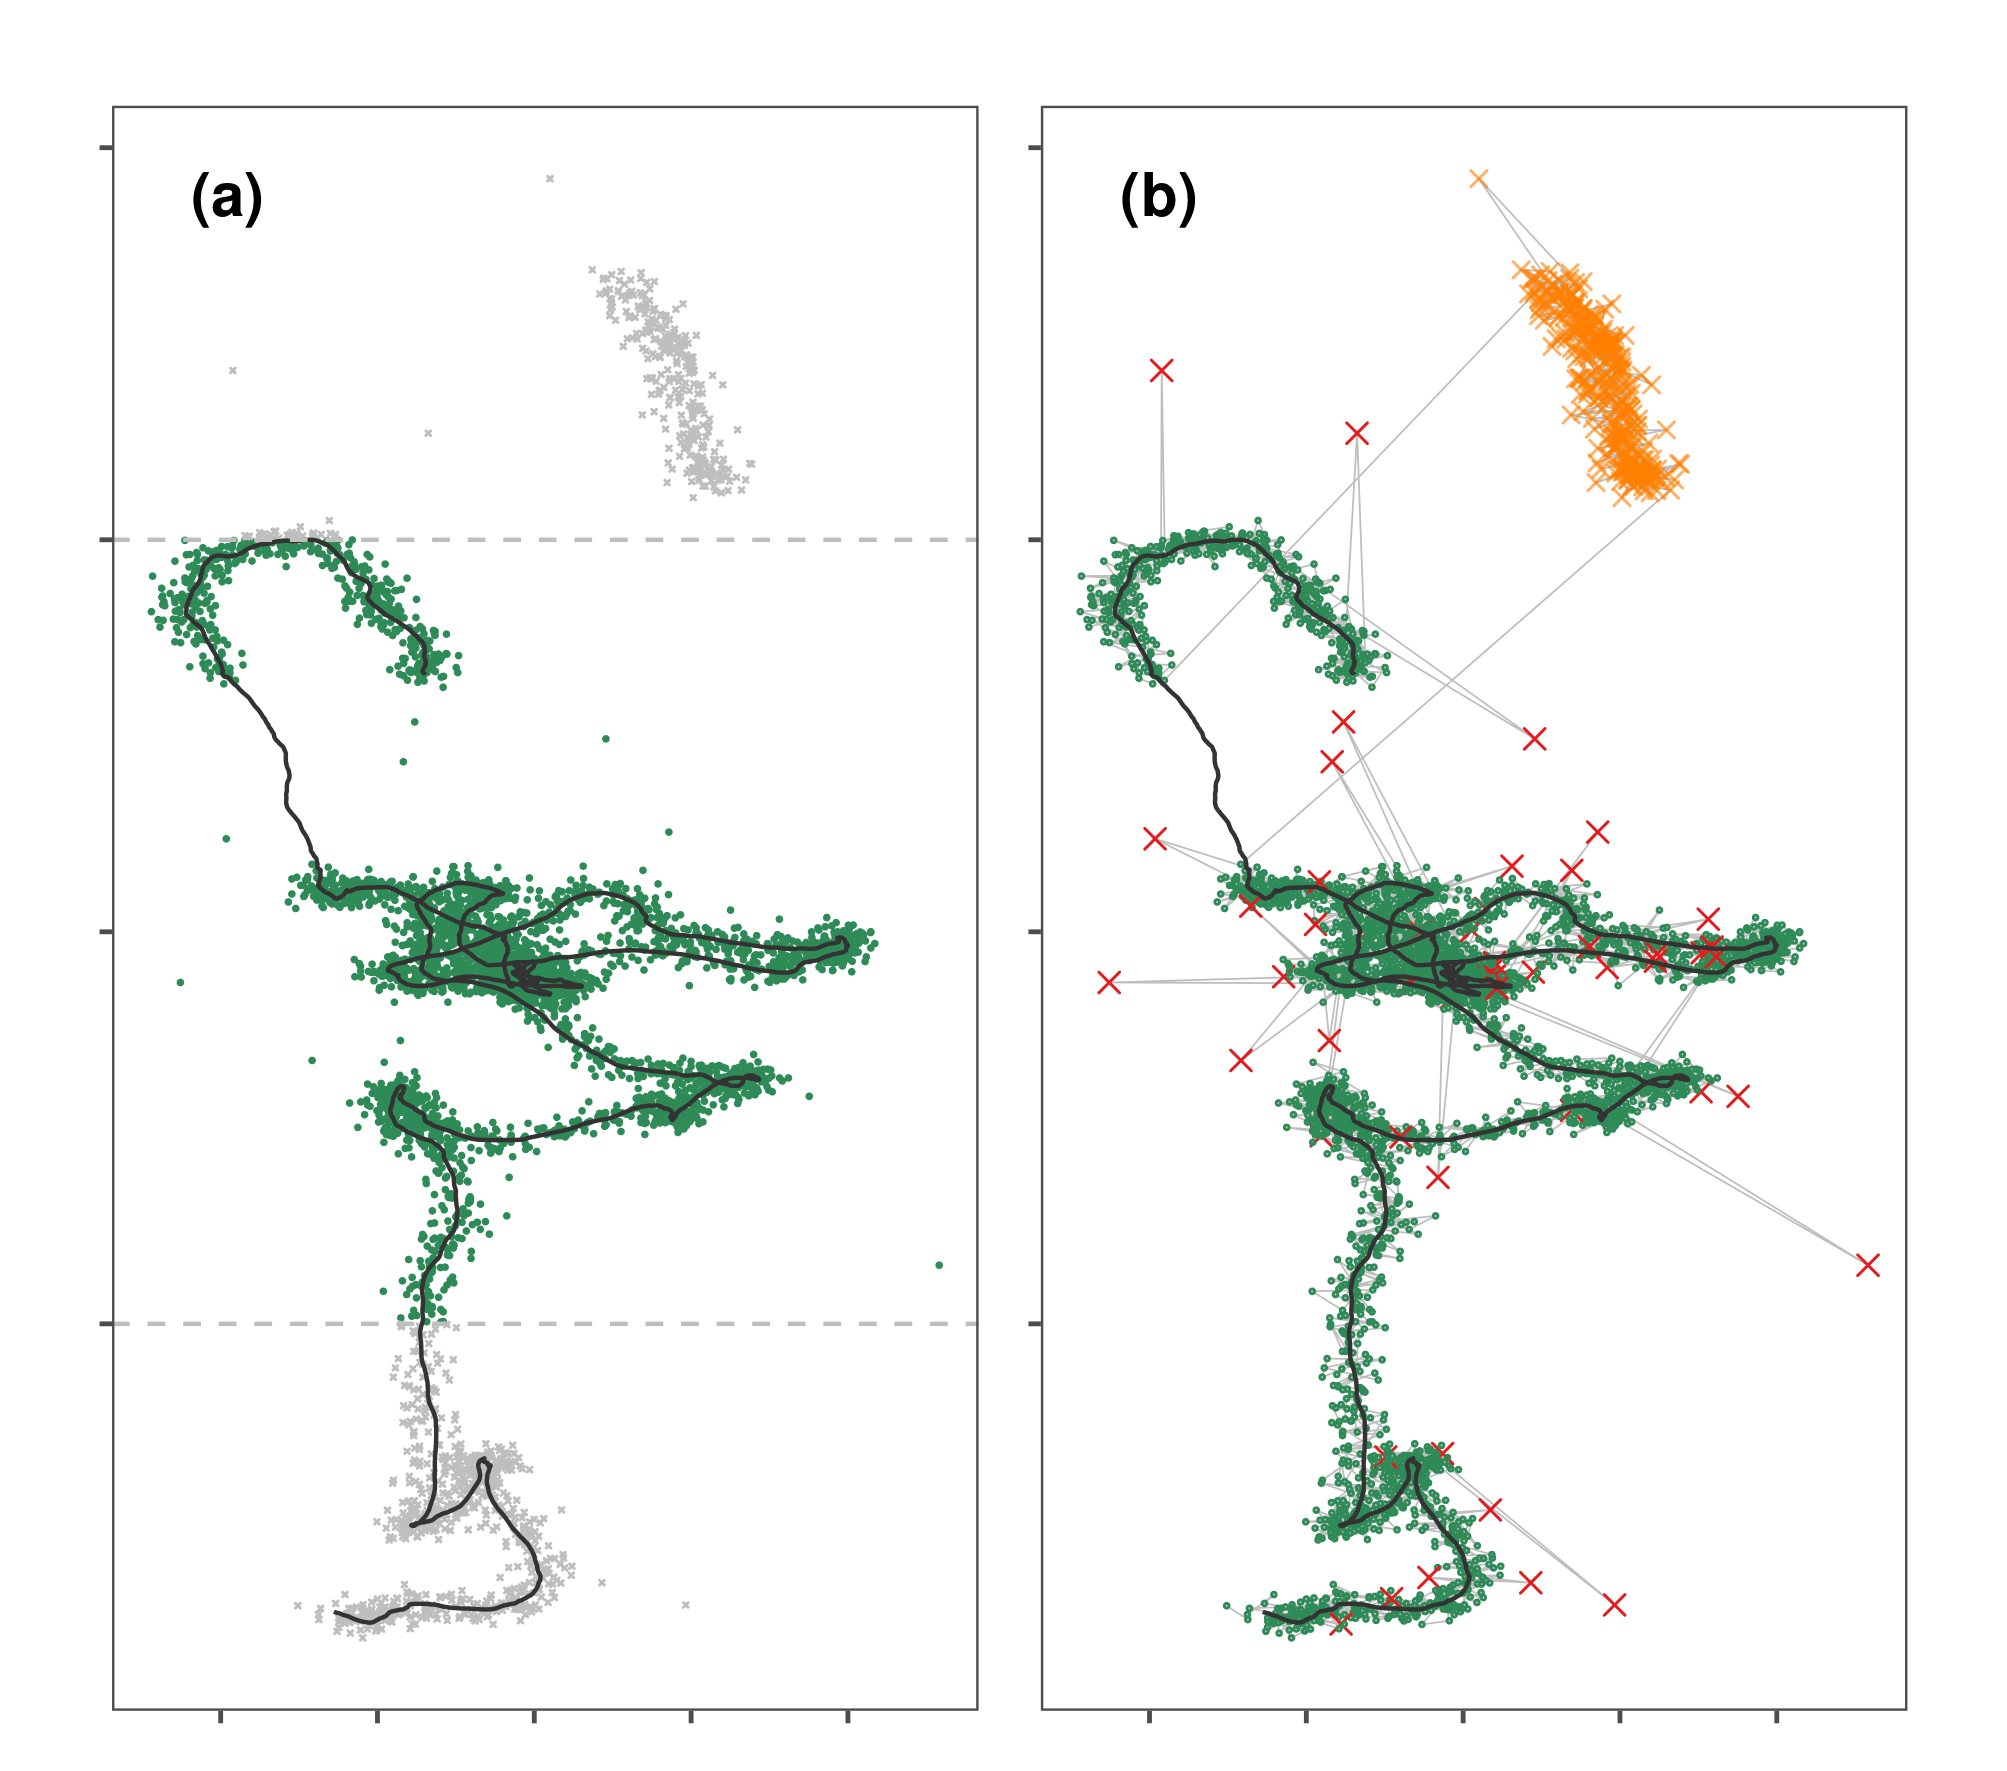
\includegraphics[width=0.95\textwidth]{figures/fig_02_filtering_data.png}
    \caption{\textbf{(a)} Simulated movement data (black line), with three kinds of artificially added errors: (1) normally distributed small-scale error on each position, (2) large-scale error added to 0.5\% of positions, and (3) 300 consecutive positions displaced to simulate a gross distortion affecting a continuous subset of the track.  
    Tracks can be quickly filtered by spatial bounds (dashed grey lines) to exclude broad regions.
    \textbf{(b)} 
    Location error may affect single observations resulting in point outliers or `spikes' (grey crosses), or continuous subsets of a track, called a `prolonged spike' (black crosses, top right), and both represent unrealistic movement.
    While spikes can be removed by filtering out positions with high incoming and outgoing speeds and turning angle, prolonged spikes cannot be effectively corrected by targeting each coordinate pair in isolation.
    These and other distortions that affect continuous track segments can be removed by conceptualising algorithms that find the bounds of the distortion and remove points in between them.
    Users should frequently check the outputs of such algorithms to avoid rejecting valid data.
    }
    \label{fig:figure_filtering_data}
\end{figure}

\subsection{Temporal and Spatio-temporal Filters}

Temporal filtering can exclude positions from periods during tracking when data are expected to be unreliable, either due to abnormal movement behaviour or poor tracking quality. 
An animal’s movement may be non-representative when it has been fitted with a tracker but has not been released, leading to artificial stationary positions, or in the time shortly after release when its movement may be influenced by the stress of capture and handling (see example implementation in \texttt{amt}; \citet{signer2019}). 
In these cases, all positions from a short time after release (e.g. 24 hours) can be excluded. 
Periods of poor tracking quality may result from system malfunctions, and temporal filters can be applied to exclude such chunks from the datastream. 
Temporal filters can be combined with spatial filters to exclude time-location combinations which would be unrealistic for the tracked animal. 
For example, red knots in the Dutch Wadden Sea congregate at communal roosts during high-tide, when their foraging grounds on the inter-tidal mudflats are inaccessible \citep{vangils2006}.
A spatio-temporal filter that retains positions inside the bounds of roosts during high-tide can quickly return data that reveals individual presence at high-tide roosts, while excluding positions that erroneously place individuals on the inundated mudflats.
% Howevever, in this example, such a filter would also exclude potentially exploratory movements over the flooded mudflats.
% We caution users to be certain that filters do not exclude positions that reveal interesting aspects of their animals' movement.
Users should apply filters in sequence rather than all at once, and visualise the output after each filtering step (`sanity checks').

The atlastools function \texttt{atl\_filter\_covariates} allows convenient filtering of a dataset by any number of logical statements (Listing 2).
This function can be used to easily filter timestamps in a range, as well as combine simple spatial and temporal filters.
It accepts a character vector of \texttt{R} expressions that each return a logical vector (i.e., \texttt{TRUE} or \texttt{FALSE}; Listing 2).
The function returns only those data which satisfy each of the filter conditions. 
Users must ensure that the filtering variables exist in their dataset in order to avoid errors.

\begin{lstlisting}[float, language=R, style=customR, caption = {
    The \texttt{atl\_filter\_covariates} function can be used both as a simple temporal filter, and also as a combined spatio-temporal filter. 
    Filter predicates are passed to the \texttt{filters} argument as a character vector, each of which is then evaluated as an \texttt{R} expression in the context of the data supplied. 
    Only rows in the data satisfying all the conditions passed as filters are retained. 
    Users must make sure the filter variables exist in their dataset.
    Here, the first example shows how nighttime data can be retained using a predicate (\texttt{inrange} from \texttt{data.table}) that determine whether the value of `hour' is between 6 and 18. 
    The \texttt{!} sign indicates that the negative of the predicate should be returned, i.e., \texttt{TRUE} when the hour is between 6 PM and 6 AM, but \texttt{FALSE} when the hour is between 6 AM and 6 PM.
    The second example shows the use of multiple filter statements; this data will be filtered to be within the range of times bounded by \texttt{t\_min} and \texttt{t\_max}, and with X coordinates between \texttt{x\_min} and \texttt{x\_max}.
    The \texttt{between} function is from \texttt{data.table}.}]
night_data <- atl_filter_covariates(data = dataset,
                filters = c("!inrange(hour, 6, 18)"))

data_in_area <- atl_filter_covariates(data = dataset,
                    filters = c("between(time, t_min, t_max)",
                                "between(x, x_min, x_max)"))
\end{lstlisting}

\section{Filtering to Reduce Location Errors}

\subsection{Filtering on Quality Covariates}

Tracking data covariates can be good indicators of the reliability of calculated positions (Beardsworth et al. \textit{in prep.}).
For intance, in ATLAS systems the number of base stations involved in each localisation is an indirect indicator of data quality, and positions localised using more receivers are usually more reliable \citep[the minimum required for an ATLAS localisation is 3; see][]{weiser2016}.
GPS systems' location error may be similarly indicated indirectly by the number of satellites involved in the localisation, or directly by an error measure such as the Horizontal Dilution of Precision (HDOP).
ATLAS and other TOA systems also calculate direct measures of location error during localisation: \texttt{VARX}, \texttt{VARY}, and \texttt{COVXY}, which are the variance of the X and Y coordinates, and the covariance of the X and Y coordinates, respectively \citep{maccurdy2009, maccurdy2019, weiser2016}.
A location error measure associated with each coordinate pair (similar to GPS HDOP) can be calculated and assigned to a new column \texttt{SD} using the formula for the sum of correlated random variables
\begin{linenomath*}
    \begin{equation*}
        SD = \sqrt{{VARX} + {VARY} + 2 \times {COVXY}}
     \end{equation*}
\end{linenomath*}
Filtering on the position-specific standard deviation allows removing unreliable positions, and the filter can be applied using \texttt{atl\_filter\_covariates}.

\begin{lstlisting}[float, language=R, style=customR, caption = {
    Filtering ATLAS data on position covariates. 
    The \texttt{filters} argument accepts a character vector with the logical statements. 
    The function only retains data for which \textit{all} the conditions are satisfied; here that is positions calculated using $>$ 3 base stations (\texttt{NBS}), with location error (\texttt{SD}) $<$ 100, and data between an arbitrary day 5 and day 8.}]
filtered_data <- atl_filter_covariates(data = data,
                    filters = c("NBS > 3",
                                "SD < 100",
                                "between(day, 5, 8)"))
\end{lstlisting}

\subsection{Filtering Unrealistic Movement}

Filtering on system-generated measures of error may not result in the removal of all erroneous positions, and data may remain which would require biologically implausible movement.
Users are encouraged to visualise their tracks before and after filtering point locations, and especially to `join the dots' and connect consecutive positions with lines.
Whether the resulting track looks realistic is ultimately a subjective human judgement, but one which implicitly integrates prior knowledge of the movement ecology of the study species to ask, `Does the animal move this way?'.
Segments which appear to represent unrealistic animal movement are often obvious to researchers with extensive experience of the study system \citep[the non-movement approach; see][]{bjorneraas2010}.
Since it is both difficult and prohibitively time consuming to exactly reproduce expert judgement when dealing with large volumes of tracking data from multiple individuals, some automation is necessary.
Users should first manually examine a representative subset of tracks and attempt to visually identify problems --- either with individual positions, or with subsets of the track --- that persist after basic filtering.
Once such problems are identified, users can conceptualise algorithms that can be applied to their data to resolve them.

An example of a problem with individual positions is that of point outliers or `spikes' \citep{bjorneraas2010}, where a single position is displaced far from the track (see Fig. 3.a).
Point outliers are characterised by artificially high speeds between the outlier and the positions before and after \citep[called incoming and outgoing speed, respectively][]{bjorneraas2010}, lending a `spiky' appearance to the track.
Removing spikes is simple: remove positions with extreme incoming and outgoing speeds.
Users must first define plausible upper limits for speed and turning angle for the study species \citep{calenge2009, seidel2018}.
Here, it is important to remember that speed estimates are scale-dependent; high-throughput tracking typically overestimates the speed between positions where the animal is stationary or moving slowly due to small-scale location errors \citep{ranacher2016, noonan2019}. 
Even after data with large location errors have been removed by filters, it is advisable to begin with a liberal (high) speed threshold that excludes only the most unlikely of speeds.
Estimates of maximum speed may not always be readily obtained for all species, and an alternative is to use a data-driven threshold such as the 95\textsuperscript{th} percentile of speeds from the track.
Once a speed threshold $S$ has been chosen, positions with incoming \textit{and} outgoing speeds $\geq S$ may be identified as spikes and removed.
Some species can realistically achieve speeds $\geq S$ in fast transit segments when assisted by environmental factors, such as birds with tailwinds, and a simple filter on incoming and outgoing speeds would exclude this valid data.
To avoid removing real, fast transit segments while still excluding spikes we suggest combining the speed filter with a filter on the turning angles of each position \citep[see][]{calenge2009}.
This combined filter assumes that positions in high-throughput tracking with both high speeds and large turning angles are likely to be due to location errors, since most species are unable to turn sharply at high speed.
Users can then retain only those positions whose incoming and outgoing speeds are both $< S$ which or satisfy the condition $\theta < A$, where $\theta$ is the turning angle, and $A$ is the turning angle threshold.
The removal of spikes is implemented using the \texttt{atl\_filter\_covariates} function (Listing 4).
Many other track metrics may be used to identify implausible movement and on which data may be filtered \citep{seidel2018}.

\begin{lstlisting}[float, language=R, style=customR, caption = {
    Filtering a movement track on incoming and outgoing speeds, and on turning angle to remove unrealistic movement.
    The functions \texttt{atl\_get\_speed} and \texttt{atl\_turning\_angle} are used to get the speeds and turning angles before filtering, and assigned to a column in the data (assignment of \texttt{speed\_out} is not shown).
    The filter step only retains positions with speeds below the speed threshold $S$ \textit{or} angles above the turning angle threshold $\theta$, i.e., positions where the animal is slow but makes sharp turns, and data where the animal moves quickly in a relatively straight line.}]
data$speed_in <- atl_get_speed(data,
                x = "x", y = "y",
                time = "time", type = c("in"))

data$angle <- atl_turning_angle(data,
                  x = "x", y = "y", time = "time")

filtered_data <- atl_filter_covariates(data = data,
        filters = c("(speed_in < S & speed_out < S) | angle < A"))
\end{lstlisting}

% \begin{figure}[h!]
%     \centering
%     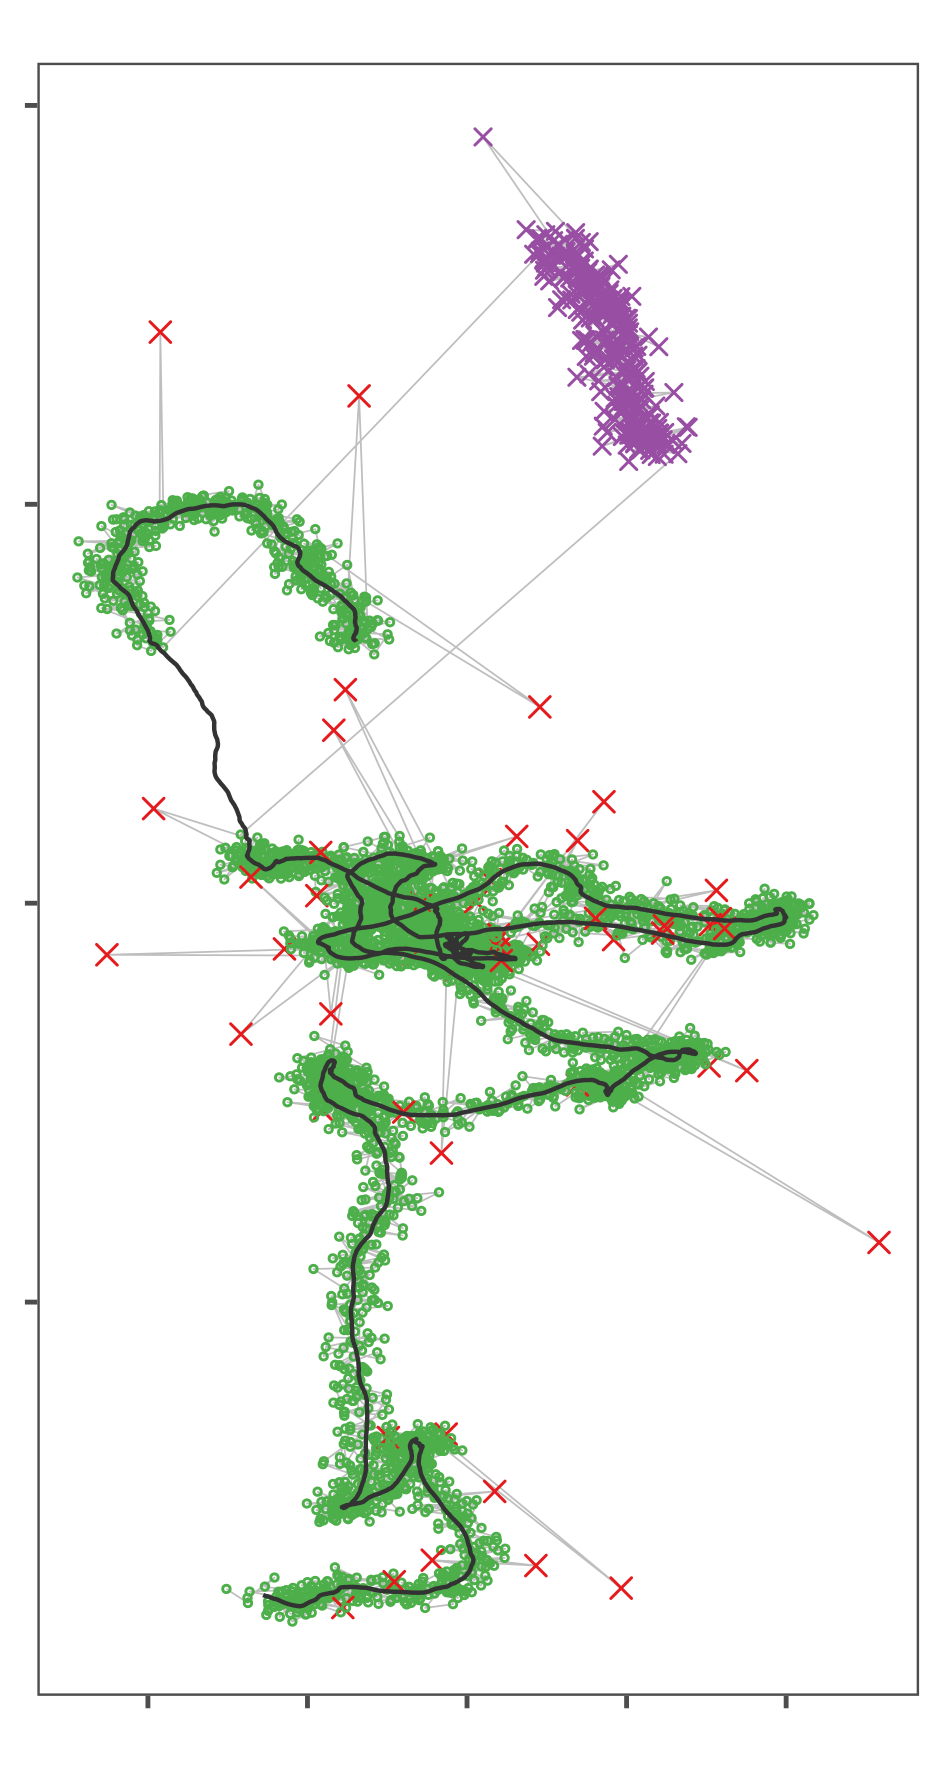
\includegraphics[width=0.95\textwidth]{figures/fig_03_filter_speed.png}
%     \caption{Reducing large-scale outliers in a movement track. The goal is to remove positions far away from the canonical track (black line), and retain those with only reasonable displacements from the canonical track (green points). 
%     \textbf{(a)} location error may affect single observations resulting in point outliers or `spikes' (grey circles), but it may also affect continuous subsets of a track, called a `prolonged spike' (purple triangles). 
%     The former may be targeted by filtering on appropriate covariates such as speed and turning angle using the \texttt{atlastools} function \texttt{atl\_filter\_covariates}.
%     Here, we filter out positions with incoming and outgoing speeds $\geq$ the 90\textsuperscript{th} percentile (0.025) and turning angle $\geq$ the 10\textsuperscript{th} percentile (35$^{\circ}$).
%     Howevever, prolonged spikes cannot be effectively corrected by targeting each coordinate pair in isolation.
%     \textbf{(b)} The \texttt{atlastools} function \texttt{atl\_remove\_reflections} to remove prolonged spikes (grey circles) in tracking data is an example of targeting track subsets with a common distortion (here, a geometric translation).
%     While this method filters out the prolonged spike to return only positions with reasonable displacement from the canonical track (green points) in this example, conceptualising and implementing such algorithms is difficult. 
%     Users are cautioned to frequently check this and similar methods' results.}
%     \label{fig:figure_filter_bounds}
% \end{figure}

Sometimes entire susbets of the track may be affected by the same large-scale location error.
For instance, multiple consecutive positions may be roughly translated (geometrically) away from the real track and form `prolonged spikes', or `reflections' (see Fig. 3.a, b).
These cannot be corrected by targeted removal of individual positions, as in Bjorneraas and colleagues' approach (2010), since there are no positions with both high incoming and outgoing speeds.
Since filtering individual positions will not suffice, algorithms to correct such errors must take a track-level view, and target the displaced sequence overall.
Track-subset algorithms are likely to be system-specific, and may be challenging to conceptualise or implement.
In the case of prolonged spikes, one relatively simple solution is identifying the bounds and removing positions between them.
We show an illustrative example of such an algorithm in the form of track-subset filtering for prolonged spikes using the \texttt{atlastools} function \texttt{atl\_remove\_reflections} (Listing 5).
Users are strongly encouraged to visualise their data before and after applying this method, and we caution against relying on this method if data are heavily distorted by errors affecting entire track-subsets.

\begin{lstlisting}[float, language=R, style=customR, caption = {
    Removing prolonged spikes from a movement track. 
    The important function arguments here are \texttt{point\_angle\_cutoff} ($A$), \texttt{reflection\_speed\_cutoff} ($S$), and \texttt{est\_ref\_len}, the maximum number of positions after the inner bound that are candidates for the end of the prolonged spike, i.e., the outer bound. 
    If the prolonged spike ends after less than $N$ positions, the true end point is used as the outer bound of the spike.
    However, the algorithm behind this function fails when the prolonged spike ends after more than $N$ positions. 
    Users are advised to use a liberally large value of N in the \texttt{est\_ref\_len} argument; 1,000 may be appropriate for 3s interval data.
    Further, users are cautioned against relying on such algorithms for severely distorted data.}]
filtered_data <- atl_remove_reflections(data = track_data,
                       x = "x", y = "y", time = "time",
                       point_angle_cutoff = A,
                       reflection_speed_cutoff = S,
                       est_ref_len = N)
\end{lstlisting}

\section{Smoothing and Thinning Data}

\subsection{Median Smoothing}

After filtering out large location errors may, the track may still look ‘spiky’ at small scales, and this is due to smaller location errors.
These smaller errors are challenging to remove since their covariates (such as speed and turning angles) are within the expected range of movement behaviour for the study species. 
The large data volumes of high-throughput tracking allow users to resolve this problem by smoothing the positions. 
A ‘smooth’ works by approximating the value of an observation based on neighbouring values.
For a one-dimensional series of observations, the neighbouring values are the $K$ observations centred on each index value $i$.
The range $ {i - (K-1)/2} \ldots {i + (K-1)/2} $ is referred to as the moving window as it shifts with $i$, and $K$ is called the moving window size.
A common smooth is nearest neighbour averaging, in which the value of an observation $x_i$ is the average of the moving window $K$.
The median smooth is a variant of nearest neighbour averaging which uses the median rather than the mean, and it is robust to outliers (\citeauthor{tukey1977} 1977).
The median smoothed value of the X coordinate, for instance, is
\begin{linenomath*}
    \begin{equation*}
        X_i = Median(X_{i - (K-1)/2} \ldots X_{i + (K-1)/2})
     \end{equation*}
\end{linenomath*}
Users can apply a median smooth with an appropriate $K$ independently to the X and Y coordinates of a movement track to smooth it (see Fig. 4.a -- e). 
% The first and last $(K - 1)/2$ values for a moving window size of $K$ are assigned a value using Tukey's (1977) end-point smoothing rule as implemented in \texttt{R} \citep{hardle1995}.
The median smooth is robust to even very large temporal and spatial gaps, and does not interpolate between positions when data are missing. 
Thus it is not necessary to split the data into segments separated by periods of missing observations when applying the filter (see Fig. 4).

Smoothing does not change the number of observations, but does decouple the coordinates from some of their covariates.
For instance, smoothing breaks the relationship between a coordinate and the location error estimate around it (\texttt{VARX}, \texttt{VARY}, and \texttt{SD} in ATLAS systems, or HDOP in GPS tracking).
This makes subsequent filtering on covariates of data quality unreliable, and smoothed data are unsuitable for use with methods that model location uncertainty \citep{noonan2019, fleming2014a, fleming2020, calabrese2016}.
Furthermore, while larger $K$ may result in smoother tracks (Fig. 4.b -- e), one drawback of using a large $K$ is that short, quick forays away from the main track are likely to be smoothed away, leading to a loss in detail of the individual's small-scale movement.
Users must themselves judge how best to trade large-scale and small-scale accuracy, and choose $K$ accordingly.
One empirical way to compare $K$ is by calculating the root mean squared error (RMSE) for different $K$ on the same data.
% In general, large $K$s lead to unrealistic tracks, both because the first and last $(K - 1) / 2$ positions are handled as special cases, and because the local median approaches the global median at larger $K$.
Median smoothing is provided by the \texttt{atlastools} function \texttt{atl\_median\_smooth}, with the only option being the moving window size, which must be an odd integer (Listing 6).

\begin{lstlisting}[float, language=R, style=customR, caption = {
    Median smoothing a movement track using the function \texttt{atl\_median\_smooth} function with a moving window \textit{K = 5}. 
    Larger values of $K$ yield smoother tracks, but $K$ should always be some orders of magnitude lower than the number of observations.}]
atl_median_smooth(data = track_data,
                  x = "x", y = "y",
                  time = "time",
                  moving_window = 5)
\end{lstlisting}

% median smooth figure
\begin{figure}[h!]
    \centering
    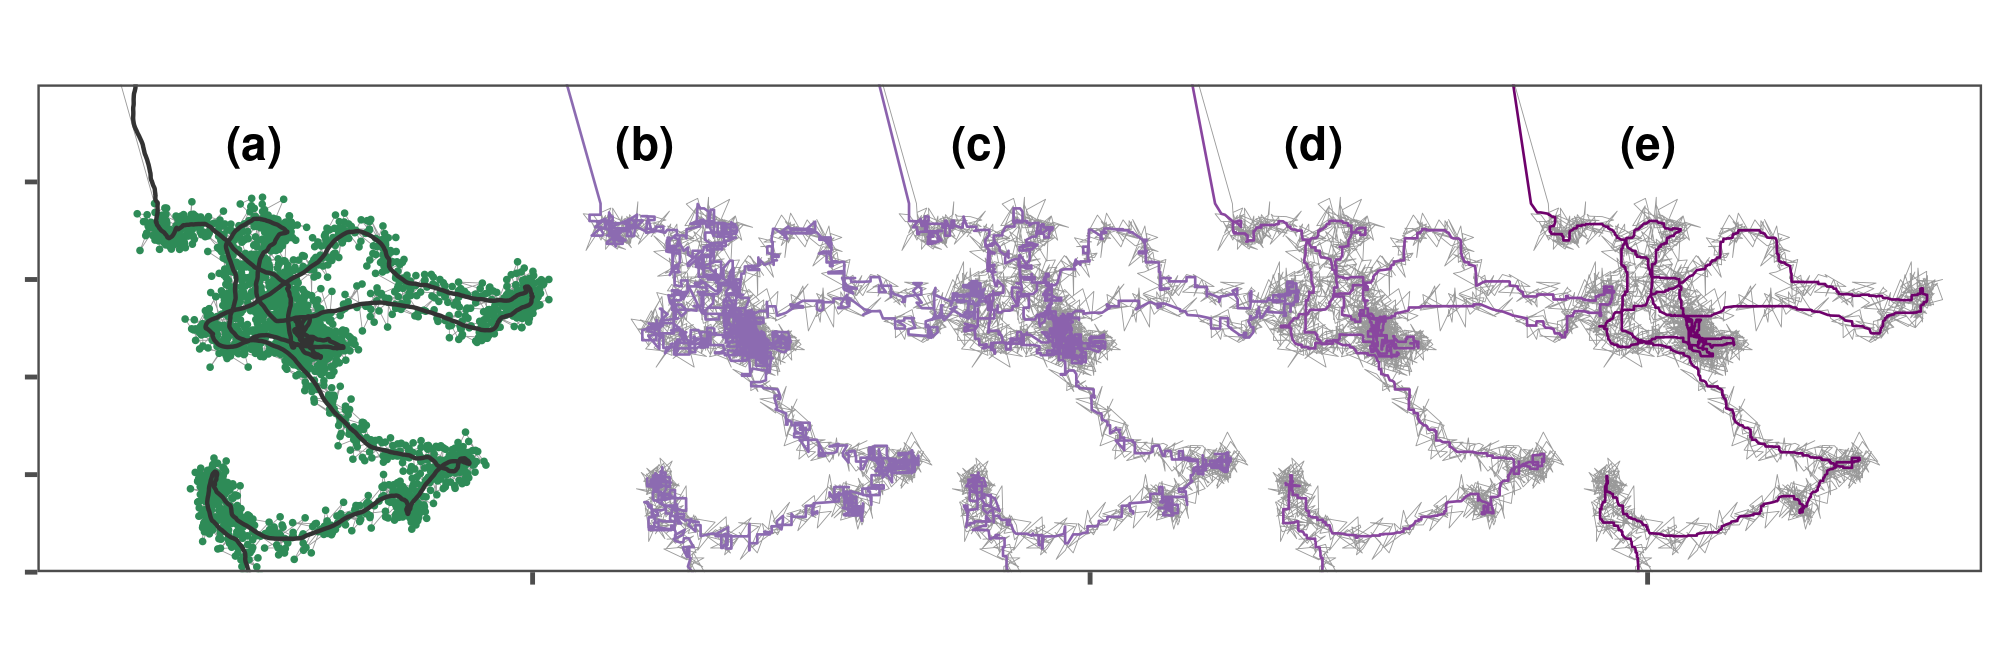
\includegraphics[width=0.95\textwidth]{figures/fig_03_median_smooth.png}
    \caption{Median smoothing position coordinates reduces small-scale location error in tracking data. 
    \textbf{(a)} The goal of this step is to approximate the simulated canonical track (black line), given positions with small-scale error remaining from previous steps (green points). 
    The canonical track is shown `zoomed in' for better representation, and the missing data at the top of the track (line with no points) is from where the prolonged spike was earlier removed.
    Median smoothing the given position coordinates ((a) green points) over a moving window ($K$) of \textbf{(b)} 3, \textbf{(c)} 5, \textbf{(d)} 11, and \textbf{(e)} 21 positions respectively, yields approximations (purple lines) of the canonical track.
    Users are cautioned that there is no correct $K$, and they must subjectively choose a $K$ which most usefully trades small-scale details of the track for large-scale accuracy.}
    \label{fig:figure_median_smooth}
\end{figure}

\subsection{Thinning Movement Tracks}

Most data at this stage is technically ‘clean’, yet its volume alone may pose challenges for lower-specification or older hardware and software if these are not optimised for efficient computation.
Thinning data need not compromise researchers' ability to answer scientific questions with them; for instance, social interactions lasting 1 -- 2 minutes would still be detected on thinning from a sampling interval of 1 second to 1 minute.
Indeed, temporal auto-correlation may hinder some methods such as the estimation of home-ranges or step-selection functions \citep{fleming2014a, dupke2017}.
Added to the requirement of uniform sampling intervals by many methods in the field, evenly reducing data volumes is a worthwhile endeavour \citep[e.g.][]{fleming2014a, michelot2016, avgar2016}.
Two plausible approaches here are resampling and aggregation, and both approaches begin with identifying time-interval groups (e.g. of 1 minute).
Resampling picks one position from each time-interval group.
Aggregation involves computing the mean values of all covariates for positions within a time-interval group.
Both approaches yield one position per time-interval group.
Categorical variables, such as the habitat type associated with each position can be aggregated using a suitable measure such as the mode.

The aggregation method is less sensitive to selecting point outliers by chance than resampling.
When users want to account for location error with methods such as state-space models \citep{jonsen2003, jonsen2005, johnson2008}, or continuous time movement models \citep{fleming2014a, noonan2019, gurarie2017, calabrese2016, fleming2020}, correctly propagating the location error when thinning is important.
In ATLAS systems the location error (\texttt{SD}; see \textsc{Filtering on Position Covariates}) is calculated from the variance-covariance matrix of the coordinates of candidate positions considered by the location solver \citep{weiser2016}; this is equivalent to GPS systems' HDOP \citep{ranacher2016}.
The error around each coordinate (\texttt{VARX} or \texttt{VARY} in ATLAS systems) can be propagated to the averaged position as the sum of errors divided by the square of the number of observations contributing to each average ($N$):
\begin{linenomath*}
    \begin{equation*}
        Var(X)_{agg} = \left( \sum_{i=1}^{i=N} Var(X)_i \right) / N ^ 2
    \end{equation*}
\end{linenomath*}
Similarly, the overall location error estimate for the average of $N$ positions in a time-interval can be calculated by treating it as a variance ($SD ^ 2$):
\begin{linenomath*}
    \begin{equation*}
        SD_{agg} = \sqrt{ \left( \sum_{i=1}^{i=N} SD_i^2 \right) / N ^ 2  }
    \end{equation*}    
\end{linenomath*}

Users may question why thinning should be implemented after cleaning steps, when aggregation can obtain consensus positions over an interval, correctly propagate the location error, and also reduce data volumes.
We caution users that thinning causes an extensive loss of small-scale detail in the data.
Additionally, thinning prior to excluding unrealistic movement and smoothing can lead to estimates of essential metrics --- such as speed --- that are substantially different from the true value (Noonan et al. 2019; see Fig. 5.c).
The mis-estimation of track metrics could have knock-on consequences for the implementation of subsequent filters based on detecting unrealistic movement.
However, thinning before data-cleaning may have its place as a useful step before exploratory visualisation of the movement track, since reduced data volumes are easier to handle for plotting software.

Thinning is implemented in \texttt{atlastools} using the \texttt{atl\_thin\_data} function, with either aggregation or resampling (specified by the \texttt{method} argument) over an interval using the \texttt{interval} argument.
The column of timestamps must be named `time' and column classes except the identity columns (\textit{see below}) should allow averaging.
The `resample' option returns a thinned dataset with all columns from the input data, but `aggregate' drops \texttt{COVXY}, as this cannot be propagated.
Using `resample' returns the actual timestamp (in UNIX time) of each sample, while `aggregate' returns the mean timestamp (also in UNIX time).
In both cases, an extra column \texttt{time\_agg} is added which has a uniform difference between each element corresponding to the user-defined thinning interval.
Due to its development for ATLAS systems, the `aggregate' assumes the variance around coordinates is named \texttt{VARX} and \texttt{VARY}, and standard deviation around each position is named \texttt{SD}.
These columns must be present together for the function to correctly handle the error.
If there is no measure of error, the function simply returns the averaged position and covariates in each time interval.
Grouping variables' names (such as animal identity) may be passed as a character vector to the \texttt{id\_columns} argument (Listing 7).

\begin{lstlisting}[float, language=R, style=customR, caption = {Code to thin data by aggregation in \texttt{atlastools}. The method can be either "aggregate" or "resample". 
The time interval is specified in seconds, while the \texttt{id\_columns} allows a character vector of column names to be passed to the function, with these columns used as identity variables.
Both methods return a dataset with as many rows as there are time-intervals.
While the resampling method retains all columns, the aggregation method drops the ATLAS specific columns specifying covariance in X and Y coordinates (COVXY), and location error (SD).}]
thinned_data <- atl_thin_data(data,
                    interval = 60,
                    id_columns = c("animal_id"),
                    method = "aggregate")
\end{lstlisting}

% figure for aggregation thinning
\begin{figure}[h!]
    \centering
    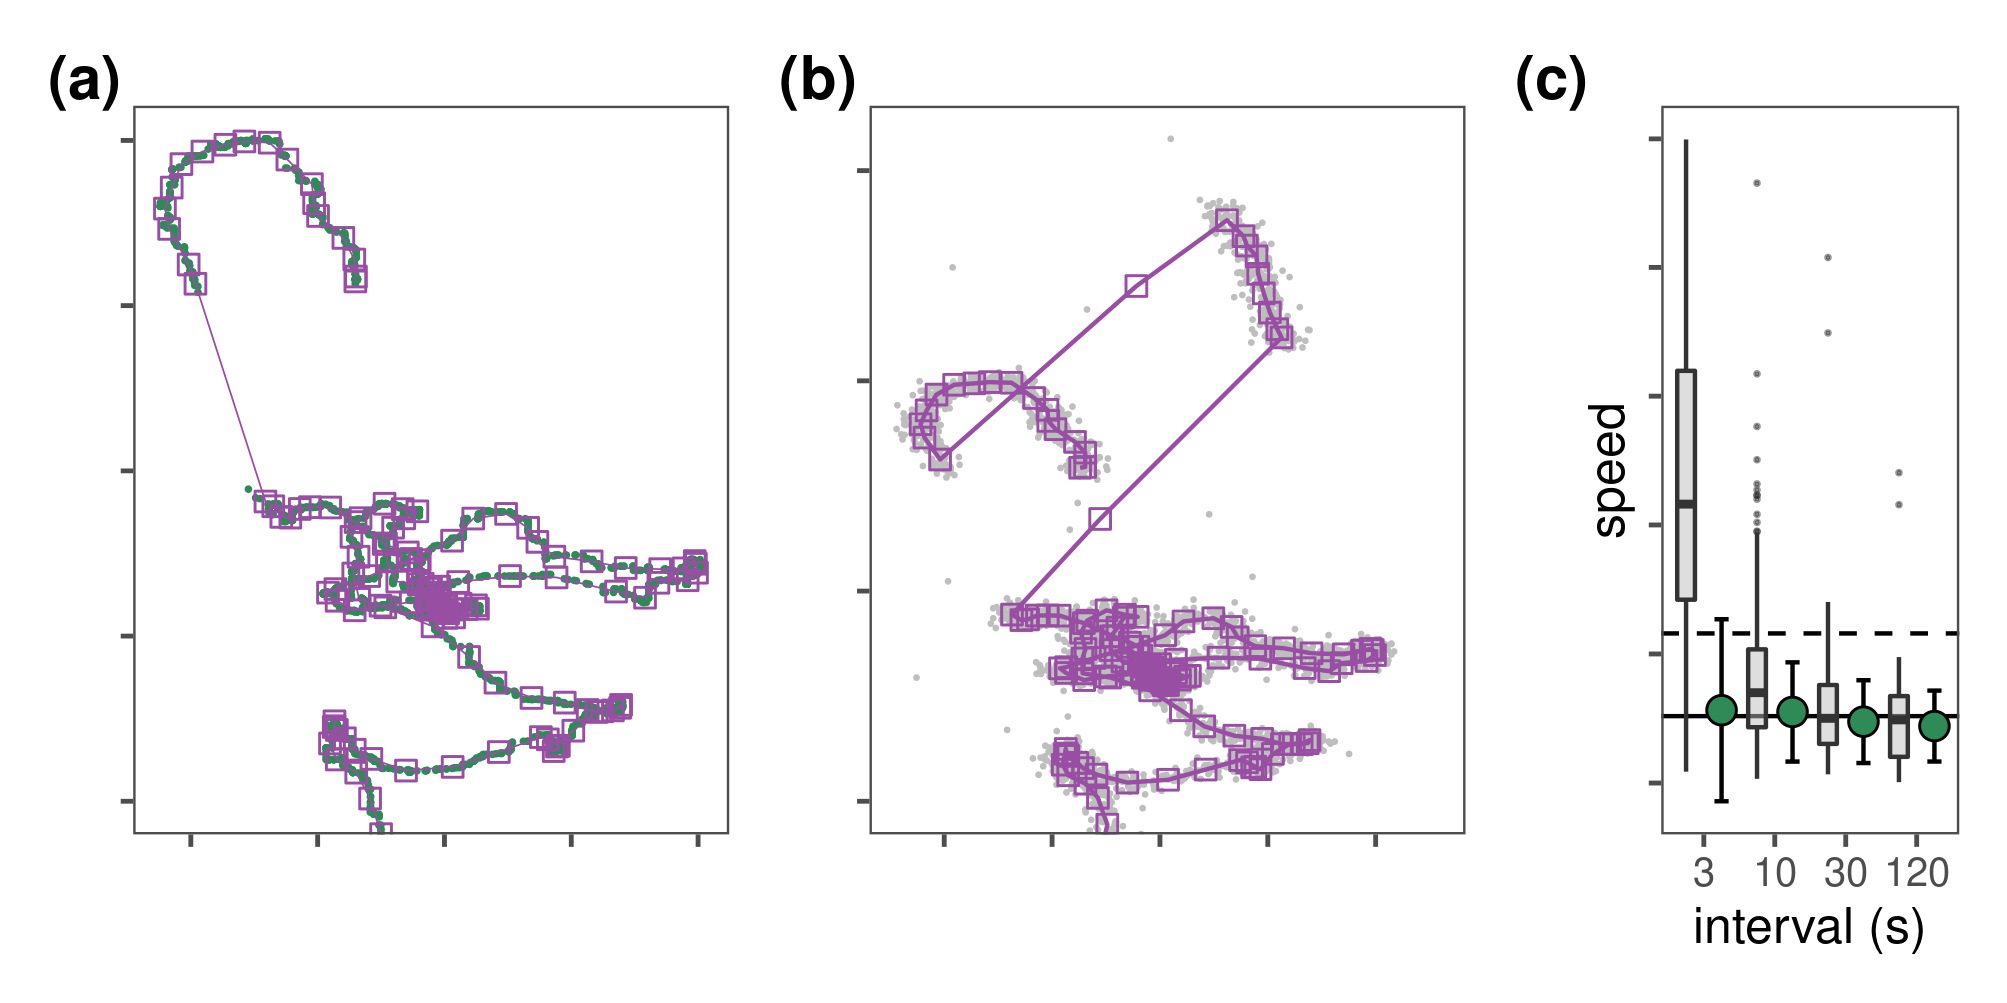
\includegraphics[width=0.95\textwidth]{figures/fig_04_thinning.png}
    \caption{\textbf{(a)} Aggregating a filtered and smoothed movement track (green points) preserves track structure while reducing data volume, but \textbf{(b)} aggregating before filtering gross location errors and unrealistic movement (grey points) leads to the persistence of large-scale errors (such as prolonged spikes).
    The thinned track is shown as purple squares and lines in both panels.
    \textbf{(c)} Thinning before data cleaning can lead to significant misestimations of essential movement metrics such as speed at lower intervals.
    Boxplots show the median and interquartile ranges for speed estimates of tracks aggregated over intervals of 3, 10, 30, and 120 seconds, but without the removal of location errors.
    For comparison, the median and 95\textsuperscript{th} percentile of speed of the canonical track are shown as solid and dashed horizontal lines, respectively.
    Green circles and associated error bars show, in contrast, the median ($\pm$ standard deviation) speed for the same aggregation interval, but after removing large- and small-scale location errors (median smooth $K$ = 11).}
    \label{fig:figure_thinning}
\end{figure}

\section{Synthesising Movement Tracks into Residence Patches}

\subsection{The Residence Patch Algorithm}

Tracking data that are still too large for statistical packages, or have strong autocorrelation, can benefit from segmentation-clustering into `residence patches' \citep{bijleveld2016, oudman2018, barraquand2008}.
Making the patch the unit of observation conveniently sidesteps pseudo-replication while and reduces computational requirements.
Furthermore, metrics such as the distance travelled within and between patches can help compare broad-scale individual movement strategies.

First, users should identify positions representing bouts of stationary behaviour, for instance on their speed or residence time \citep{bracis2018}.
Patch identification assesses whether consecutive positions and the bouts they comprise are spatio-temporally independent, and clusters them together if they are not.
The splitting and lumping of positions into bouts, and bouts into patches is based on simple user specified thresholds --- the distance and the time interval between positions (and bouts) beyond which they should be considered independent.
% Patches are considered independent if either the distance or time between them exceeds their respective thresholds.
Users are encouraged to base these thresholds in the movement habits of their study species.
For example, residence patch classification of red knot movement tracks considers consecutive stationary positions independent if they are 20m apart and considers consecutive bouts independent if the distance between them $\geq$ 100m, or the time difference between them $\geq$ 30 minutes (Listing 8).
The 20m distance represents a maximum speed of 6.667 m/s between positions, above which the individual is more likely in transit.
The 100m and 30 minute thresholds are chosen to account for potentially missing data between bouts; if a track ends abruptly and then reappears $\geq$ 100m away or $\geq$ 30 minutes later, this is more safely considered a new residence patch.

A cleaned movement track can be classified into residence patches using the function \texttt{atl\_res\_patch} (see Fig. 6.c).
\texttt{atl\_res\_patch} requires three parameters: (1) the distance threshold between positions (called \texttt{buffer\_size}), (2) the distance threshold between clusters of positions (called \texttt{lim\_spat\_indep}), and (3) the time interval between clusters (called \texttt{lim\_time\_indep}).
Clusters formed of fewer than a minimum number of positions can be excluded.
% The exclusion of clusters with few positions can help in removing bias due to short stops, but if such short stops are also of interest, they can be included by reducing the \texttt{min\_fixes} argument.
Our residence patch algorithm is capable of correctly identifying clusters of related residence points from a movement track (Fig. 7.a, 7.b).
This includes clusters where the animal is relatively stationary (orange and green patches, Fig. 7.c), as well as clusters where the animal is moving slowly (blue patch, Fig. 7.c).
This flexibility is especially useful when studying movements that may represent two different modes of the same behaviour, for instance, area-restricted search, as well as slow, searching behaviour with a directional component.

The function \texttt{atl\_patch\_summary} can be used to extract patch-specific summary data such as the median coordinates, the patch duration, the distance travelled within the patch, and the patch area.
Position covariates such as speed may also be summarised patch-wise by passing covariate names and  summary functions as character vectors to the \texttt{summary\_variables} and \texttt{summary\_functions} arguments, respectively.
Setting the \texttt{which\_data} argument to \texttt{"spatial"}, returns \texttt{sf\ MULTIPOLYGON} objects, and setting \texttt{which\_data = "points"} returns the positions in each patch, with patch-specific covariates.
% The advantage of this latter option is that it can be matched to the larger dataset of positions to more accurately calculate distances between patches.

\begin{lstlisting}[float, language=R, style=customR, caption ={The \texttt{atl\_res\_patch} function can be used to classify a track into residence patches. The arguments \texttt{buffer\_radius} and \texttt{lim\_spat\_indep} are specified in metres, while the \texttt{lim\_time\_indep} is provided in minutes. In this example, specifying \texttt{summary\_variables = c("speed")}, and \texttt{summary\_functions = c("mean", "sd")} will provide the mean and standard deviation of instantaneous speed in each residence patch. The \texttt{atl\_patch\_summary} function is used to access the classified patch in one of three ways, here using the \texttt{summary} option which returns a table of patch-wise summary statistics.}]
patches <- atl_res_patch(data = track_data,
                buffer_radius = 10,
                lim_spat_indep = 100,
                lim_time_indep = 30,
                min_fixes = 3,
                summary_variables = c("speed"),
                summary_functions = c("mean", "sd"))
              
patch_summary <- atl_patch_summary(patch_data = patches,
                    which_data = "summary",
                    buffer_radius = 10)
\end{lstlisting}

% first residence patch figure
\begin{figure}[h!]
    \centering
    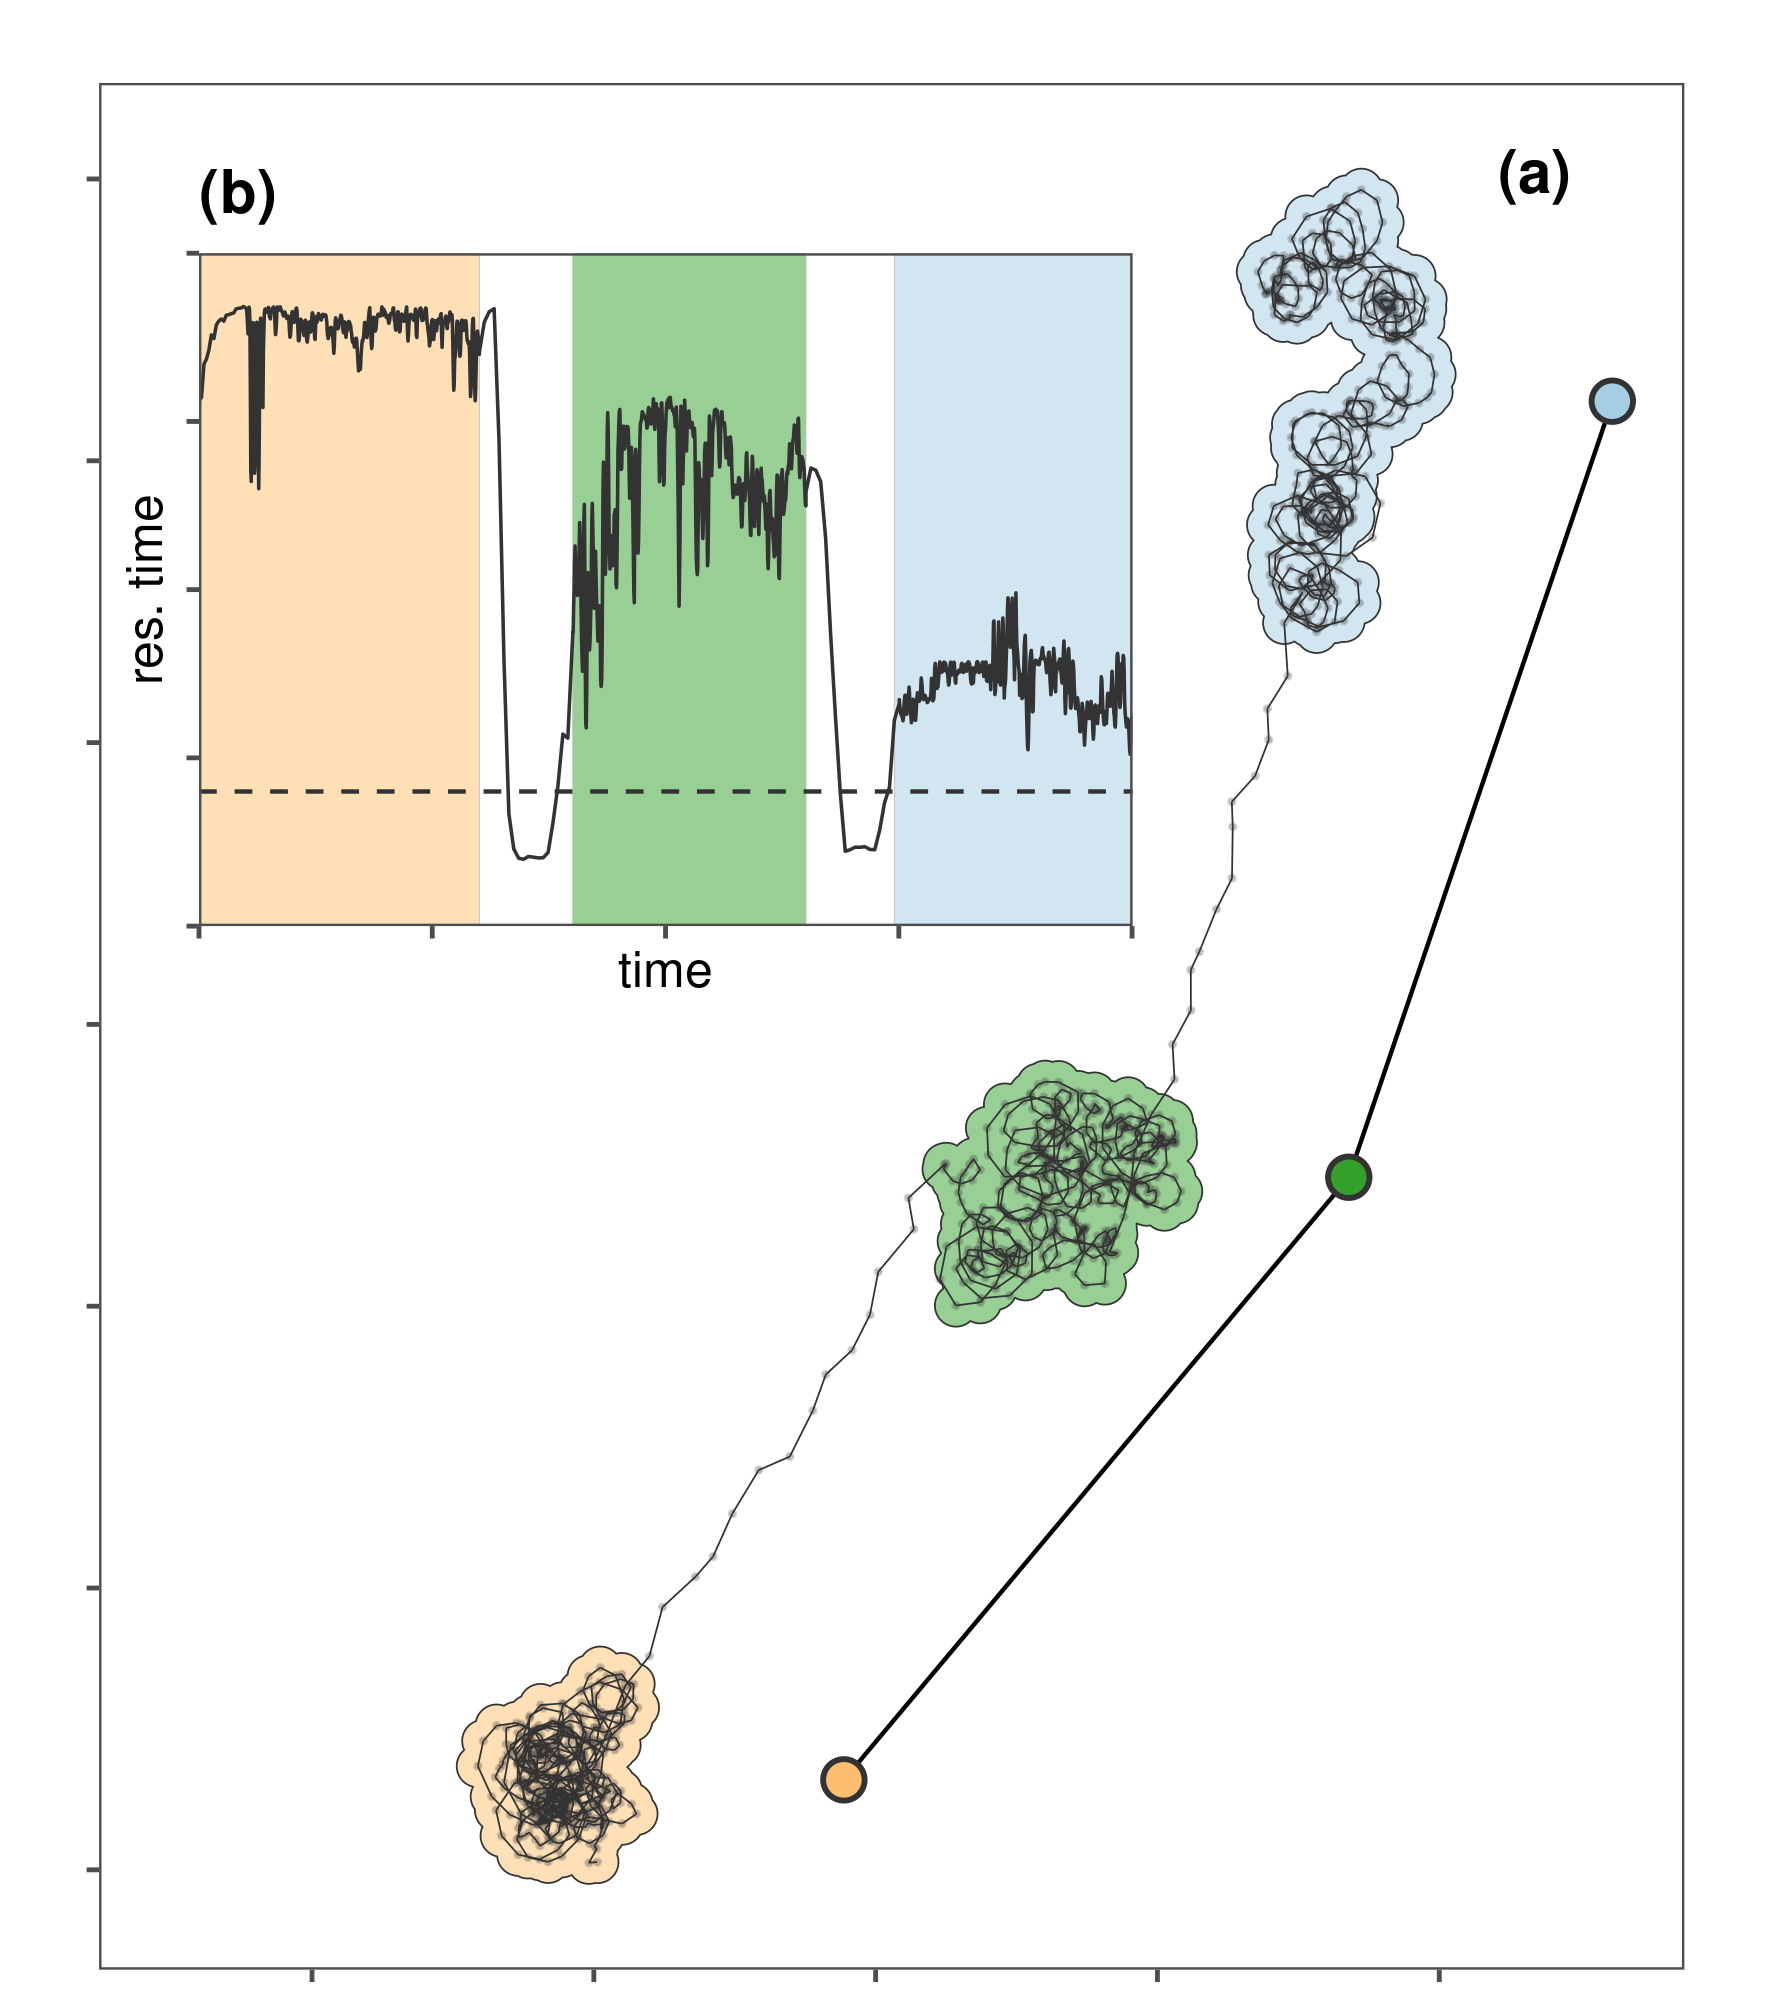
\includegraphics[width=0.75\textwidth]{figures/fig_05_residence.png}
    \caption{Movement tracks can be classified into residence patches, whcih are areas of prolonged residence (clusters of points), while leaving out the transit between them.
    \textbf{(a)} The residence patch method correctly identifies clusters of positions where the individual is relatively stationary (orange and green patches), as well as positions where it is slowly moving (blue patch).
    This is especially useful when studying more complex behaviour such as area-restricted search, which may have a directional component.
    The residence patch method loses the details of movement between patches, but can efficiently represent the general pattern of space-use (see coloured points representing patch centroids, and lines joining them).
    \textbf{(b)} A plot of residence time against time (solid line; Bracis et al. 2018) shows how the residence patch algorithm segments and clusters positions of prolonged residence. 
    Regions are shaded by the temporal bounds of each residence patch.
    The arguments passed to \texttt{atl\_res\_patch} determine the clustering, and can be adjusted to get a result that fits the study system.
    Users are cautioned that there are no `correct' arguments, and the best guide is the biology of the tracked individual.}
    \label{fig:figure_residence_patch}
\end{figure}

\subsection{Validating the Residence Patch Method}

We applied the pre-processing pipeline using \texttt{atlastools} functions described above to a calibration dataset to verify that the residence patch method could correctly identify known stopping points (see Fig. 7).
We collected the calibration data (n = 50,816) by walking and boating with a hand-held WATLAS tag (sampling frequency = 1 Hz) around the island of Griend (53.25$^{\circ}$N, 5.25$^{\circ}$E) in August 2020 (Beardsworth et al. \textit{in prep.}; Bijleveld et al. \textit{in prep.}).
Stops in the calibration track were recorded as waypoints using a handheld GPS device (Garmin Dakota 10) at each stop.
We estimated the real duration of each stop as the time difference between the first and last position recorded within 50m of each waypoint, within a 10 minute window before and after the waypoint timestamp (to avoid biased durations from revisits).
Stops had a median duration of 10.28 minutes (range: 1.75 minutes -- 20 minutes; see Supplementary Material).
We cleaned the data before constructing residence patches by (1) removing a single outlier ($>$ 15 km away), removing unrealistic movement ($\geq$ 15 m/s), smoothing the data ($K$ = 5), and (4) thinning the data by resampling over a 30 second interval.
The cleaning steps retained 37,324 positions (74.45\%), while thinning reduced these to 1,803 positions (4.8\% positions of the smoothed track).
Details and code are provided in the Supplementary Material (see \textsc{Validating the Residence Patch Method with Calibration Data}).

% We began by visualising the data to check for location errors, and found a single outlier position approx. 15km away from the study area (Fig. 7.a).
% This outlier was removed by filtering data by the X coordinate bounds using the function \texttt{atl\_filter\_bounds}; X coordinate bounds $\leq$ 645,000 in the UTM 31N coordinate reference system were removed (n = 1; remaining positions = 50,815).
% We then calculated the incoming and outgoing speed, as well as the turning angle at each position using the functions \texttt{atl\_get\_speed} and \texttt{atl\_turning\_angle} respectively, as a precursor to targeting large-scale location errors in the form of point outliers.
% We used the function \texttt{atl\_filter\_covariates} to remove positions with incoming and outgoing speeds $\geq$ the speed threshold of 15 m/s (n = 13,491, 26.5\%; remaining positions = 37,324, 73.5\%; Fig. 7.b).
% This speed threshold was chosen as 5 m/s faster than the known boat speed, 10 m/s.
% Finally, we targeted small-scale location errors by applying a median smooth with a moving window size $K$ = 5 using the function \texttt{atl\_median\_smooth} (Fig. 7.c).
% This step does not reduce the number of positions.

We identified stationary positions (residence time $\geq$ 5 minutes) using the \texttt{recurse} package \citep[n = 837, 46.42 \%; radius = 50m][]{bracis2018}.
We clustered these positions into residence patches with a buffer radius of 5m, spatial independence limit of 50m, temporal independence limit of 5 minutes, and a minimum of 3 positions per patch.
Inferred residence patches corresponded well to the locations of stops (see Fig. 7.c).
However, the residence patch algorithm detected more stops than were logged as waypoints (n = 28, n waypoints = 21).
One of these was the field station on Griend where the tag was stored between trips (red crossed-square, Fig. 7.c).
The method also did not detect two stops of 105 and 563 seconds (1.75 and 9.4 minutes) since they were data poor and aggregated away in the thinning step (n positions = 6, 15).
To determine whether the residence patch method correctly identified the duration of stops in the calibration track, we first extracted the patch attributes using the function \texttt{atl\_patch\_summary}.
We then matched the patches to the waypoints by their median coordinates (rounded to 100 metres).
We assigned the inferred duration of the stop as the duration of the spatially matched residence patch.
We compared the inferred duration with the real duration using a linear model with the inferred duration as the only predictor of the real duration.
% We excluded a single waypoint (WP080) since we had accidentally stopped there for $>$ 60 minutes.
Inferred duration was a good predictor of the real duration of a stop (linear model estimate = 1.021, t-value = 12.965, $p <$ 0.0001, $R^2$ = 0.908; see Supplementary Material Fig. 1.7).
This translates to a 2\% underestimation of the stop duration at a tracking interval of 30 seconds.

% calibration figure
\begin{figure}[h!]
    \centering
    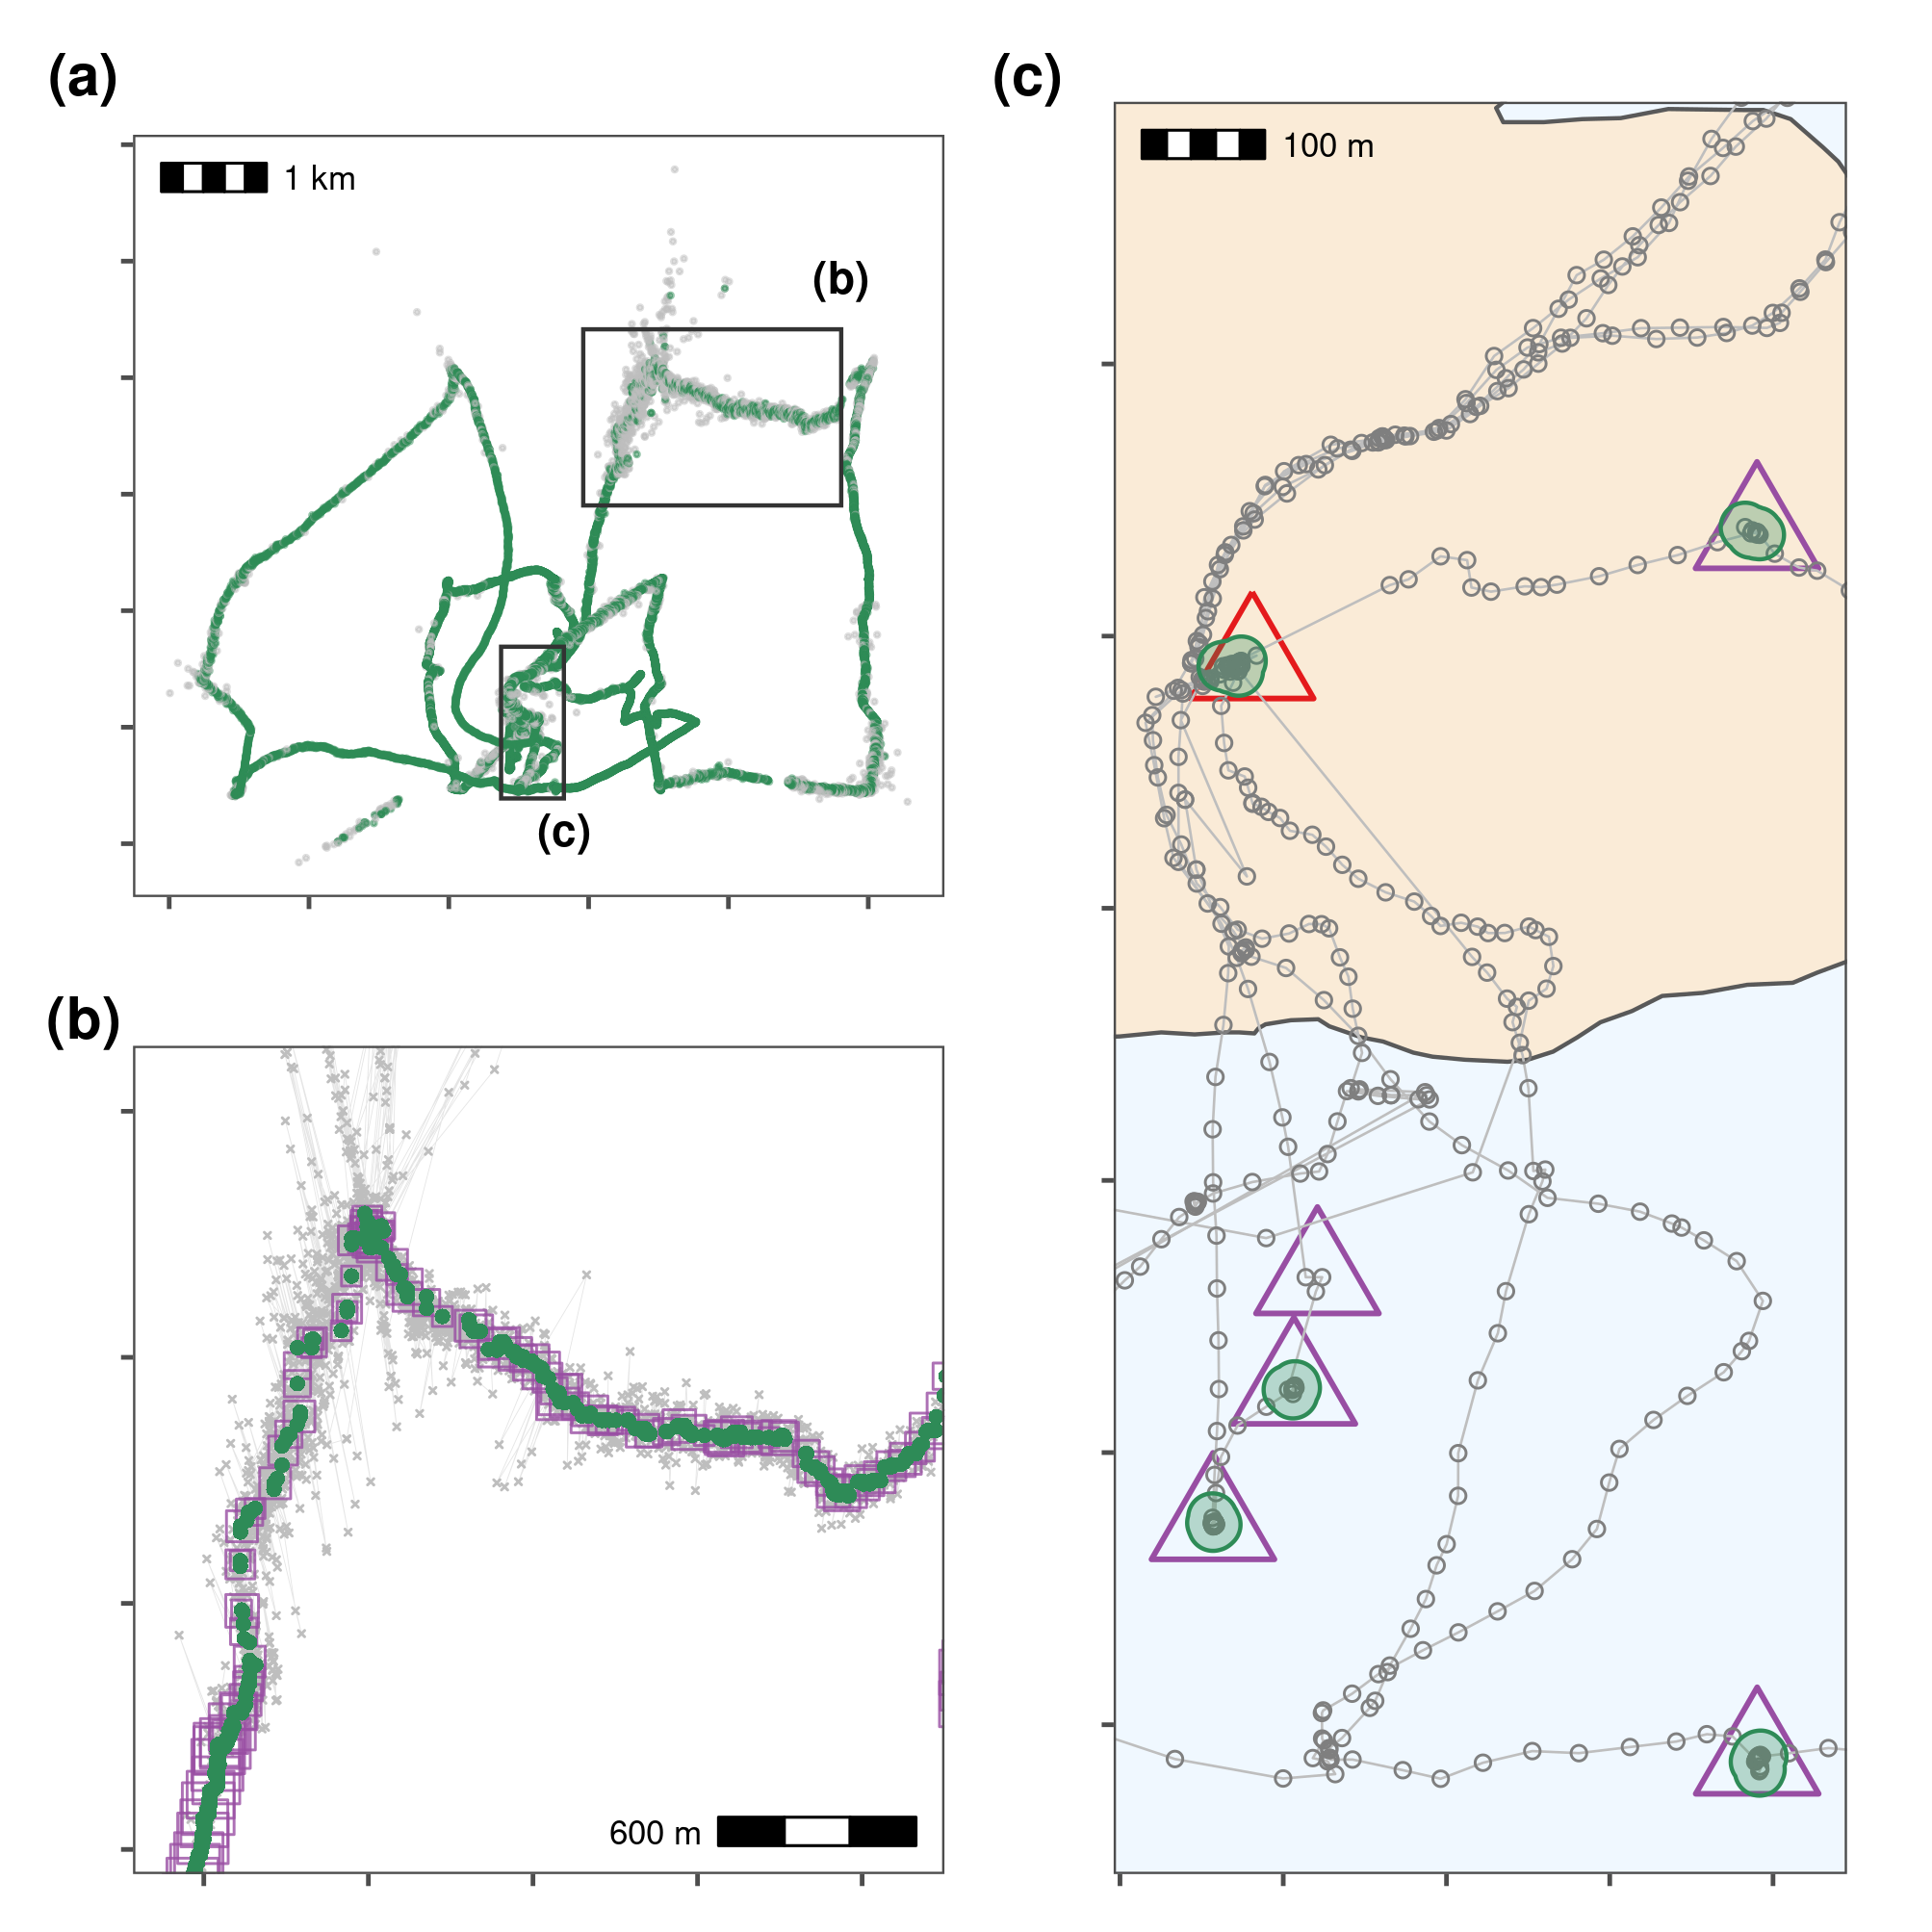
\includegraphics[width=0.75\textwidth]{figures/fig_06_calib_residence_patch.png}
    \caption{Pre-processing steps for WATLAS calibration data showing filtering filtering on speed, median smoothing and thinning by aggregation, and making residence patches.
    \textbf{(a)} Positions with incoming and outgoing speed $\geq$ the 15 m/s are removed (N removed = 13,491, 26.6\%; grey crosses = removed, green points = retained).
    Rectangles show the region expanded in subfigures (b) and (c).
    \textbf{(b)} Expanded view of upper rectangle in (a) showing the raw data (grey crosses), the median smoothed positions (green circles; moving window $K$ = 5), and the smoothed track thinned by aggregation to a 30 second interval (purple squares).
    Square size corresponds to the number of positions used to calculate the averaged position during thinning, with no significant differences.
    Median smoothing retains all 37,324 observations (though changing their coordinates). Thinning aggregates these positions into 1,803 aggregates (4.8\% of the smoothed data volume).
    Median smoothing recovers a good estimate of the true track from significantly over-dispersed raw data, while thinning reduces the data volume but preserves track structure.
    \textbf{(c)} Classifying thinned data into residence patches yields robust estimates of the duration of known stops. The island of Griend (53.25$^{\circ}$N, 5.25$^{\circ}$E) is shown in beige.
    Residence patches (green polygons; function parameters in text) correspond well to the locations of known stops (purple crossed-squares).
    However, the algorithm identified all areas with prolonged residence, including those which were not intended stops, such as stops at the field station (n = 12; green polygon over red crossed-squares).
    The algorithm also failed to find two stops of 6 and 15 seconds duration, since these were lost in the data thinning step (crossed-square without green polygon shows one of these).}
    \label{fig:figure_calibration}
\end{figure}

\section{Worked-Out Example on Animal Tracking Data}

We present a fully worked-out example of our pre-processing pipeline and residence patch method using movement data from three Egyptian fruit bats tracked using the ATLAS system (\textit{Rousettus aegyptiacus}; \citet{toledo2020}).
Code can be found in the Supplementary Material (see \textsc{Processing Egyptian Fruit Bat Tracks}).
Bats were tracked over three nights (5\textsuperscript{th}, 6\textsuperscript{th}, and 7\textsuperscript{th} May, 2018) in the Hula Valley, Israel (33.1$^{\circ}$N, 35.6$^{\circ}$E), with an average of 13,370 positions (SD = 2,173; range = 11,195 -- 15,542; interval = 8 seconds) per individual.
Plotting the tracks showed severe distortions (see Supplementary Material Fig. 2.1).
We first reduced location errors by removing observations with ATLAS SD $>$ 20, and observations calculated using fewer than four base stations (mean positions remaining = 10,447 / individual; 78\% of the raw data on average).
% We converted the ATLAS time format (milliseconds since the UNIX Epoch) to the more common UNIX format (seconds since the Epoch) by taking the floored value of the time divided by 1000.
We removed unrealistic movement represented by positions with incoming and outgoing speeds $>$ 20 m/s leaving 10,337 positions per individual on average (98\% of previous step).
We median smoothed the data with a moving window $K$ size = 5, and no observations were lost.

We began the construction of residence patches by finding the residence time within 50 metres of each position \citep{bracis2018}.
Bats may repeatedly traverse the same routes, and this could artificially inflate the residence time of positions along these routes.
To avoid confusing revisits with residence, we limited the summation of residence times at each position to the period until the first departure of 60 minutes or more.
Thus, two nearby locations ($\leq$ 50m apart) each visited for one minute at a time, but separated by an interval of some hours would not have a residence time of two minutes each, but only one minute each.
Bats had a mean residence time at locations of 100.54 minutes (SD = 114.7); this measure was strongly biased by time spent at the roost.
We opted for a first-principles approach and selected as residence positions any locations with a residence time $>$ 5 minutes, reasoning that a flying animal stopping for $>$ 5 minutes at a location should plausibly indicate resource use or another interesting behaviour.
This step retained 7,819 positions per bat on average (75.6\%) of the smoothed data; suggesting the extent to which roosting biases the data.

We constructed residence patches with a buffer distance of 25m, a spatial independence limit of 100m, a temporal independence limit of 30 minutes, and rejected patches with fewer than three positions.
We extracted summary data and spatial polygons from the constructed residence patches.
Plotting the bats' residence patches and the linear paths between them showed that though all three bats roosted at the same site, they used distinct areas of the study site (Fig. 9.a).
Bats tended to show prolonged residence near known food sources (fruit trees), travelling repeatedly between previously visited areas (Fig. 9.b).
However, bats also appeared to spend some time at locations where no fruit trees were recorded, prompting questions about their use of other food sources, or another behaviour entirely (Fig. 9.b, 9.c).
Bats occurring close together did not have strongly overlapping residence patches, and their paths to and from area of co-occurrence were different (Fig. 9.a, 9.c).
Constructing residence patches for multiple individuals over multiple nights suggests interesting dynamics of within- and between-individual overlap.

\begin{figure}[h!]
    \centering
    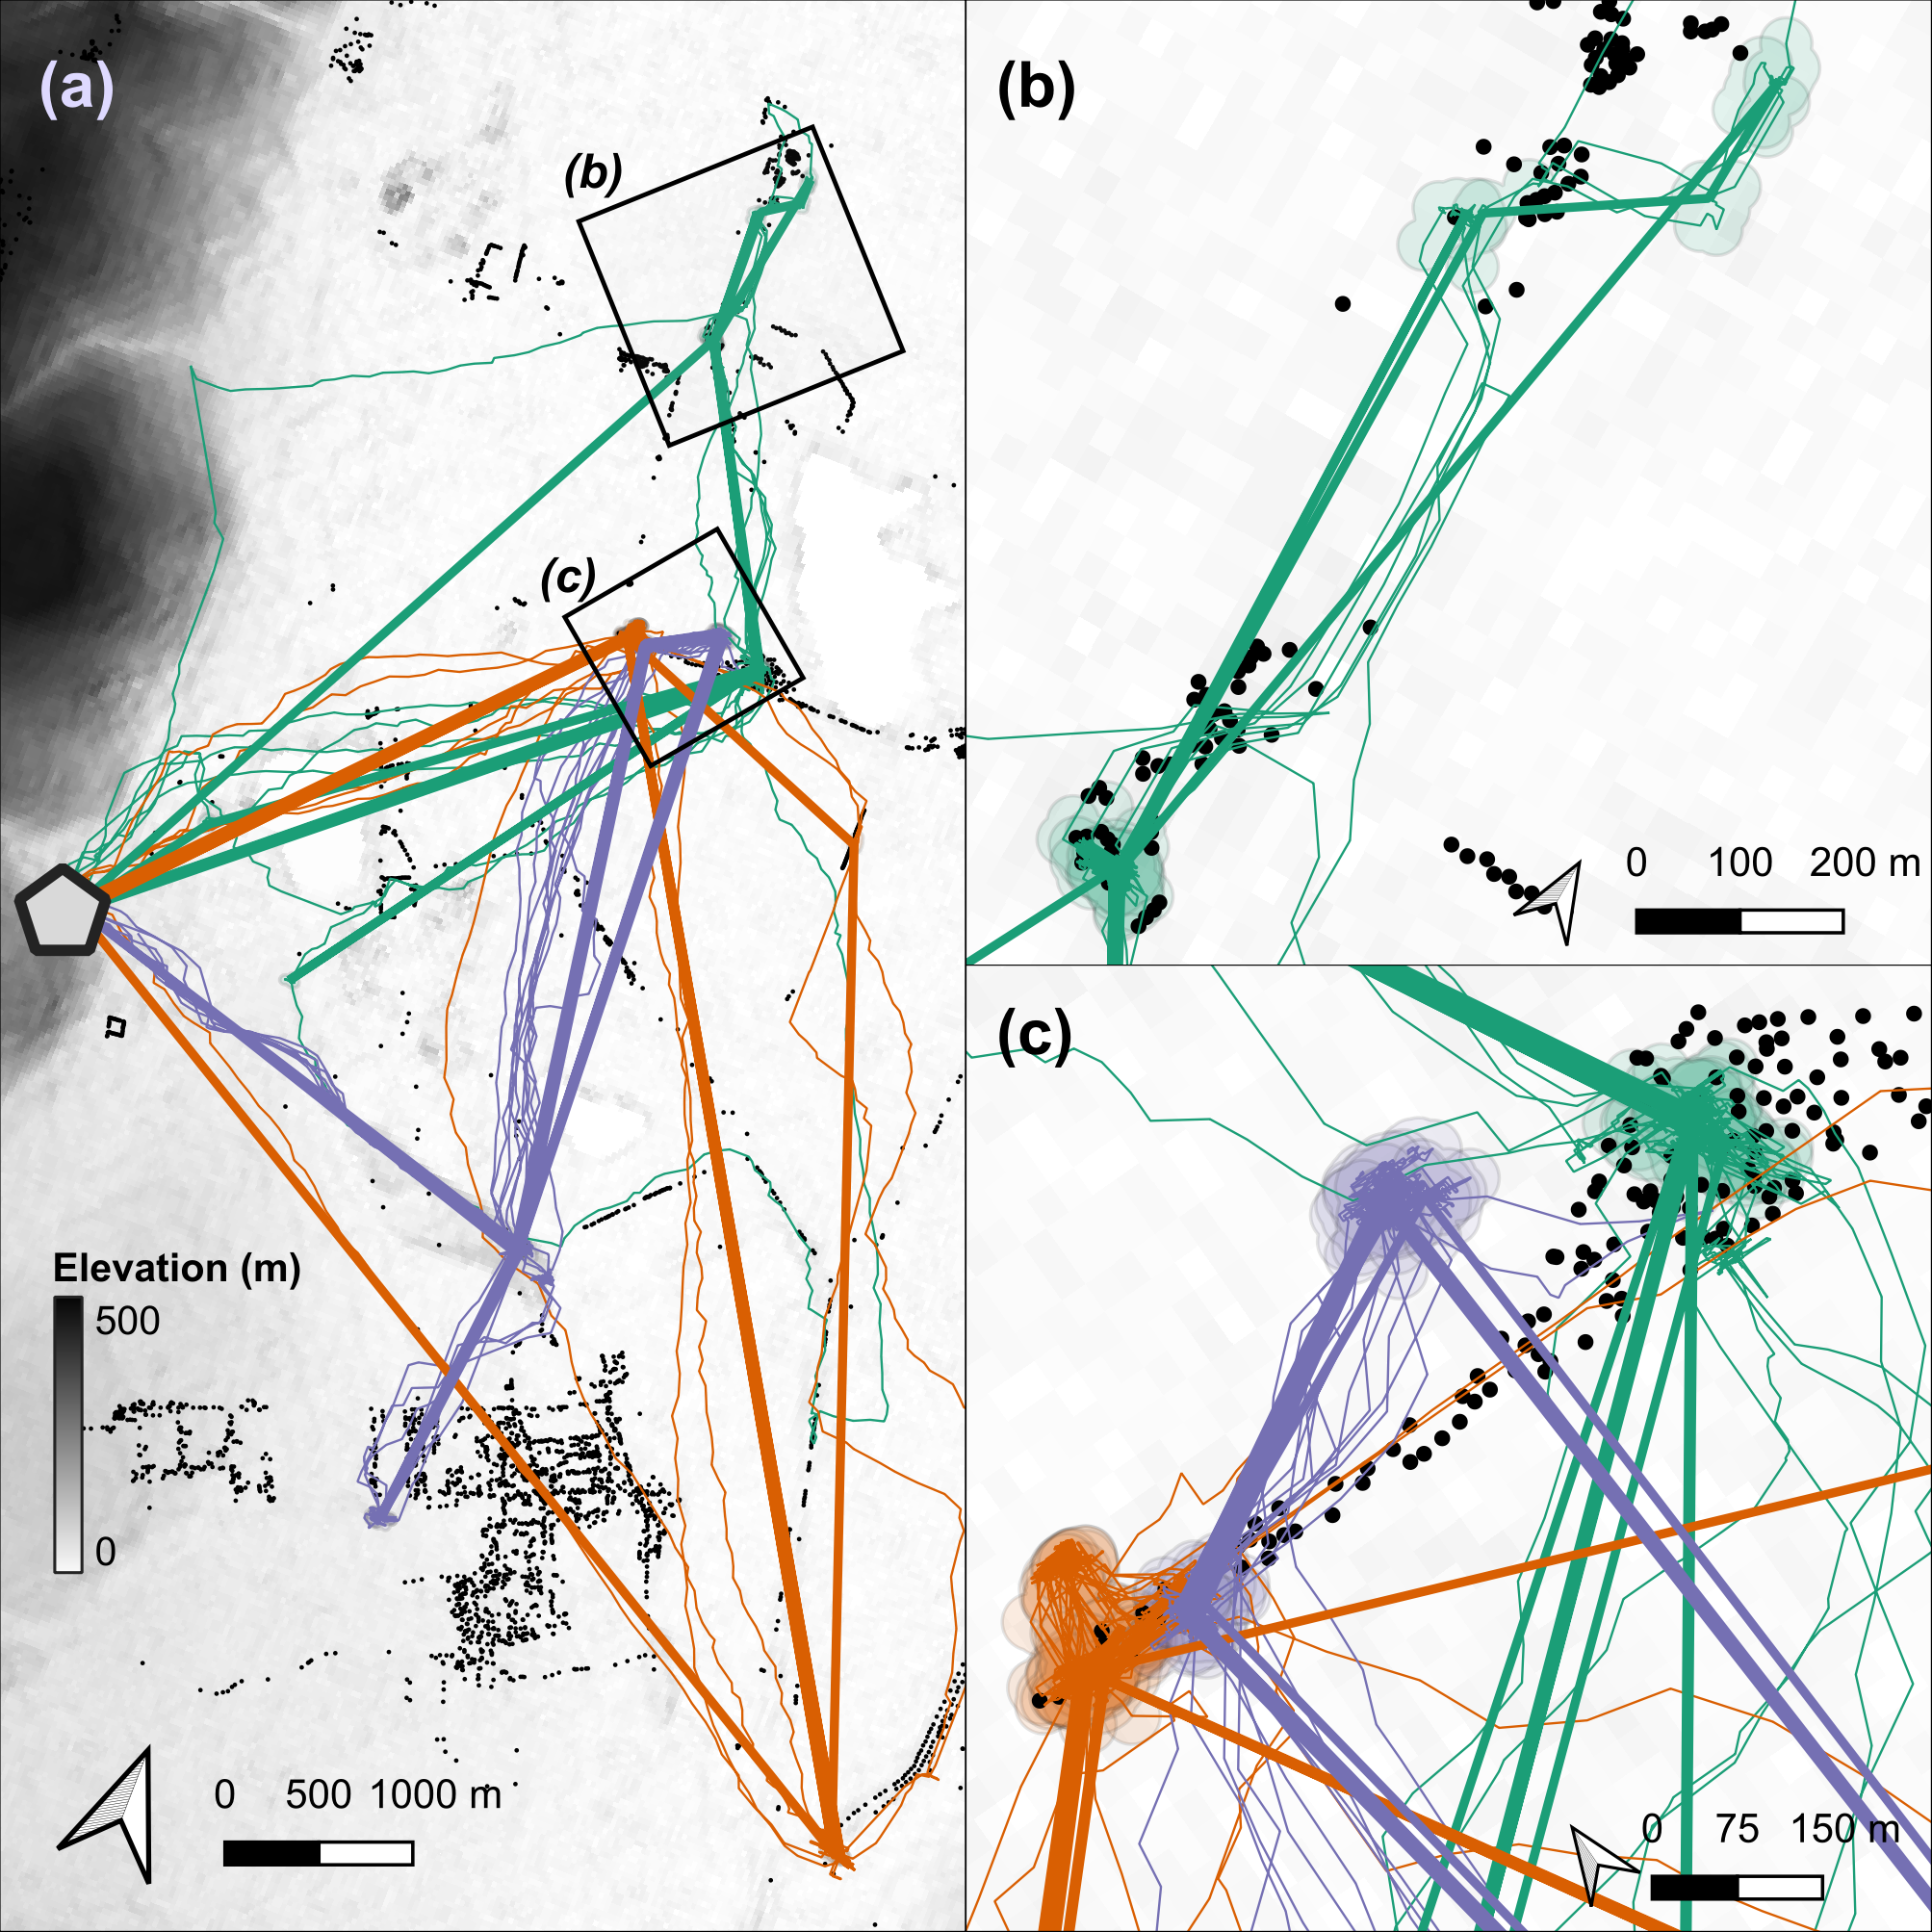
\includegraphics[width=0.75\textwidth]{figures/fig_07_bats.png}
    \caption{Synthesising animal tracks into residence patches can reveal how individuals in a population move in relation to landscape features, prior exploration, and other individuals.
    \textbf{(a)} Linear approximations of the paths (coloured lines) between residence patches (circles) show the movement of three Egyptian fruit bats (\textit{Rousettus aegyptiacus}), tracked over three nights in the Hula Valley, Israel.
    Bat tracks are are shown as thin lines below the linear approximations.
    Colours show bat identity. The grey hexagon represents a roost site.
    Dark green points represent known fruit trees.
    Background is shaded by elevation at 30 metre resolution (SRTM).    
    \textbf{(b)} Spatial representations of an individual bat's residence patches (green polygons) can be used to study site-fidelity by examining overlaps between patches, or to study resource selection by inspecting overlaps with known resources (here, black circles show the location of clusters of fruit trees).
    In addition, the linear approximation of movement between patches (blue paths in panel (a)) can be contrasted with the estimated real path between patches (green lines).
    \textbf{(c)} Residence patch polygons can also show how individuals partition space and resources (black circles are fruit trees), and the combined influence of resource and potential social cues on movement between patches (coloured paths).
    Patches and paths are coloured by bat identity.}
    \label{fig:figure_bats}
\end{figure}

\section{Discussion}

Our guide anticipates high-throughput animal tracking data becoming increasingly common.
A uniform pipeline and toolset for data cleaning promotes reproducibility and standardisation across studies, making comparative inferences more robust.
The open-source \texttt{R} package \texttt{atlastools} serves as a starting point for methodological collaboration among movement ecologists.
Efficient location error modelling approaches \citep{fleming2020} may eventually make data-cleaning optional.
Yet cleaning tracking data even partially before modelling location error will be faster than error-modelling on the full data, and the removal of large location errors may improve model fits.
Thus we see our pipeline as complementary to these approaches \citep{fleming2014a,fleming2020}.
Finally, we recognise that the diversity and complexity of animal movement and data collection techniques often requires bespoke pre-processing solutions.
Though the principles outlined here are readily generalised, users' requirements will eventually exceed the particular tools we provide.
We see this as an incentive for more users to be involved in developing methods for their systems.
We offer our pipeline and package as a foundation for system specific tools in the belief that simple, robust concepts are key to methods development that balances system-specificity and broad applicability.

%%%%%%%%%%%%%%%%%%%%%%%%%%%%%%%%%%%%%%%%%%%%%%
%%                                          %%
%% Backmatter begins here                   %%
%%                                          %%
%%%%%%%%%%%%%%%%%%%%%%%%%%%%%%%%%%%%%%%%%%%%%%
\section{Backmatter}

\subsection{Competing Interests}

The authors declare that they have no competing interests.

\subsection{Acknowledgements}

PRG would like to thank Pedro M. Santos Neves for introducing PRG to \texttt{R} package development, for help with setting up \texttt{atlastools}, and for help with archiving it on Zenodo; 
Aparajitha Ramesh and Franjo Weissing for discussions on error propagation;
Geert Aarts, Jacob RL Gismann, Evy Gobbens for feedback that improved the manuscript; 
members of the Modelling Adaptive Response Mechanisms Group (Weissing Lab), and the Theoretical Biology department at the University of Groningen for helpful discussions on \texttt{atlastools} and the manuscript.
All authors thank the attendees of ATLAS workshops held in May and June 2020 at the Hebrew University of Jerusalem for helpful comments on the pipeline and \texttt{atlastools}.

\subsection{Authors' Contributions}

PRG wrote the manuscript and inline code snippets, performed the analyses, prepared the figures, and developed the \texttt{R} package \texttt{atlastools}.
CEB and AIB collected the calibration track, and EL collected the bat movement data and fruit tree locations.
RN conceived the idea of writing this manuscript, and PRG, AIB, OS, CEB, ST, and EL contributed to its design, and the design of \texttt{atlastools}.
All authors contributed to the writing of the manuscript, and the design of figures.

\subsection{Data Availability}

The data and source code to reproduce the figures and analyses in this article and in the Supplementary Material can be found in the Zenodo repository at https://doi.org/10.5281/zenodo.4287462.

\subsection{Supplementary Material}
\begin{enumerate}
    \item Supplementary Material 1: Code for worked out examples on calibration data from the Dutch Wadden Sea, and bat tracking data from the Hula Valley, Israel.
    \item Supplementary Material 2: Manual for the \texttt{R} package \texttt{atlastools}.
\end{enumerate}


%%%%%%%%%%%%%%%%%%%%%%%%%%%%%%%%%%%%%%%%%%%%%%%%%%%%%%%%%%%%%
%%                  The Bibliography                       %%
%%                                                         %%
%%  Bmc_mathpys.bst  will be used to                       %%
%%  create a .BBL file for submission.                     %%
%%  After submission of the .TEX file,                     %%
%%  you will be prompted to submit your .BBL file.         %%
%%                                                         %%
%%                                                         %%
%%  Note that the displayed Bibliography will not          %%
%%  necessarily be rendered by Latex exactly as specified  %%
%%  in the online Instructions for Authors.                %%
%%                                                         %%
%%%%%%%%%%%%%%%%%%%%%%%%%%%%%%%%%%%%%%%%%%%%%%%%%%%%%%%%%%%%%

\nolinenumbers
\singlespacing

% if your bibliography is in bibtex format, use those commands:
\bibliographystyle{amnatnat} % Style BST file (bmc-mathphys, vancouver, spbasic).
\bibliography{references.bib}      % Bibliography file (usually '*.bib' )
% for author-year bibliography (bmc-mathphys or spbasic)
% a) write to bib file (bmc-mathphys only)
% @settings{label, options="nameyear"}
% b) uncomment next line
%\nocite{label}

%%
%% Do not use \listoffigures as most will included as separate files

\clearpage
%%%%%%%%%%%%%%%%%%%%%%%%%%%%%%%%%%%%%%%%%%%%%%
%%                                          %%
%% Figures here                             %%
%%                                          %%
%%%%%%%%%%%%%%%%%%%%%%%%%%%%%%%%%%%%%%%%%%%%%%

\end{document}
